\documentclass{kththesis}

\usepackage{graphicx} % figures
\usepackage{csquotes} % Recommended by biblatex
\usepackage{biblatex}
\usepackage{mathtools}
\usepackage{listings}
\addbibresource{references-extra.bib}
\addbibresource{references.bib} % The file containing our references, in BibTeX format

\title{Robot-human handovers learning of novel objects through unsupervised learning}
\alttitle{Inlärning av robot till människa överlämningar genom unsupervised learning}
\author{Simon Simonsson}
\email{simonsim@kth.se}
\supervisor{Christian Smith}
\examiner{John Folkesson}
\programme{Master in Computer Science}
\school{School of Electrical Engineering and Computer Science}
\date{\today}

\begin{document}

\frontmatter % Frontmatter includes the titlepage, abstracts and table-of-contents
\titlepage

\begin{abstract}
	english abstract
\end{abstract}

\begin{otherlanguage}{swedish}
	\begin{abstract}
		svensk sammanfattning
	\end{abstract}
\end{otherlanguage}

\tableofcontents

\mainmatter % Mainmatter is where the actual contents of the thesis goes

\chapter{Introduction}
\section{Background}

There are many different scenarios where we could imagine we would draw advantage of a robot performing handovers to a human. In an industrial environment, to save human workers the time of fetching tools by themselves, a robot could be employed for the task of handing over the tools when needed. In another scenario a robot could be employed into helping a human with a physical disability into reaching different things around the home. Different objects require different grips and/or movements to perform the actual handover. We can not for example hand over a sharp knife the same way that we hand over a pen, nor a hammer the same way we would for a cup of hot coffee. A challenge with robot-human handovers is to get the robot to perform the handover correctly depending on the object in question. In an industrial environment the number of tools that the robot is to handover is finite, and it is possible to train it for each one the tools. Howerver in the home of someone with a disability there is almost an infinite amount of different objects that can require handovers and it would be very inefficient to train the robot for each one of them. Existing methods for determining proper handover movements relie on robot-computed configurations and preprogrammed object-specific information. These methods all require data over correct hand grip and movement connected to objects as mentioned in this article [section IV.C]. With this work we would like to propose a way for a robot to determine grasp and handover methods purely from observations, in the goal of making it able to adapt to new objects without any prior knowlegde about grasp configurations.

\section{Research Question}

In this work we want to see if we can develop a system for a robot to learn autonomisly how to handover over a series of different objects without labeling the data, and if it can apply this to novel objects that it has not seen. We will be answering questions such as if there is a way to classify handovers and if there is a link between object properties and a type of handover. Later we will see if this is applicable to new objects.

With this project we will try to answer the following questions:
\begin{itemize}
	\item Are we able to classify objects by their handover settings?
	\item Can we relate the visual aspects of an object to its class?
	\item Is this model applicable to new objects?
\end{itemize}


\chapter{Related work}
\section{Handovers}
% handovers and research around it
Object handovers is a process that involves many parameters. Object grasping, timing of social cues and head gaze are just a few to mention some. Studies suggest that humans prefer a minimum jerk, human-like motion when being handed over an object \parencite{Huber2008} \parencite{Huber2008a}. As a consequence other research has set their focus on observing humans as to identify these parameters that affect a handover and their importance, with the aim of having robots imitate humans. \textcite{Moon2014} found that only by imitating human gaze cues during a handover the robot can help the human reach for the object sooner, even before the robot finishes the movement.

\textcite{Huang2015} researched adaptation between humans in collaborative tasks, concluding that adaptively coordinating actions can increase performance in tasks such as handovers between robots and humans. The work of \textcite{Chan2015} found through a user study of handovers under different conditions that natural handovers may differ from receiver-oriented handovers, showing us that robots would need to take this into account when learning from demonstration to make sure it puts the human interests in priority.

Although \textcite{Koene2014} found through their research that a fast motion from the robot was better received from the human side than a spatially accurate end position of the robotic grasp, \textcite{Admoni2014} showed through their experiments that introducing some deliberate delays in the handover helps the receiver with focusing on the robot's head (i.e. gaze) and understand better its suggestions, which was also proposed by \parencite{Moon2014}.

\begin{figure}
	\centering
	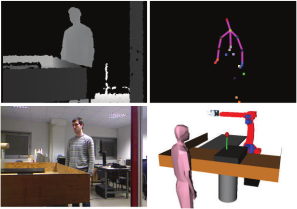
\includegraphics[width=0.5\textwidth]{img/related-work/planning-simulation.png}
	\caption{Human detection phase and handover planning in simulated environment in \parencite{Aleotti2012}.}
\end{figure}

\section{Grasping}
% grasping
A very important feature as to ensure the success of a handover, is the grasping of objects. Robotic grasping is itself a widely researched topic and several models have been proposed to compute proper grasp settings. Some examples of previous work that attempt at defining the representation of the object and its features for the task of grasping include \textcite{Miller2003} who decompose an object into primitive shapes to identify good grasping points (seen in figure \ref{fig:rel__shape-primitives}), while \textcite{Huebner2008} use a Minimum Volume Bounding Box solution to do the same (seen in figure \ref{fig:rel__mvbb}). \textcite{Morales} represent objects by nine different high level descriptors of data and developed a learning framework upon this.

Just as with handovers, in the domain of grasping several studies have been conducted as to observe human grasping as to make robots imitate them. \parencite{Cutkosky1990} \parencite{Feix2009} \parencite{Kang1993} made taxonomies for different grasp choices used by humans depending on objects and tasks. For the task of handovers, some research tried associating correct grasping of objects with their type and its affordances (\parencite{Song2015}, \parencite{Chan2014}) where by associating an object with different ways of manipulating it we identify a grip which is best suited when handing it over as to increase productivity for the receiver. Seeing how force closures are usually quite limited in terms of mobility (at least relative to the human hand), this thesis will not concentrate on the actual grasping and just leave it as future work after the correct grasping region has been identified as shown in figure \ref{fig:grasp-representation}. Please refer to the work in \parencite{Sahbani2012} for a complete review of the possibilities for robotic grasping.

\begin{figure}
	\centering
	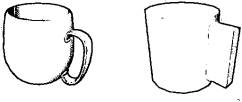
\includegraphics[width=0.3\textwidth]{img/related-work/shape-primitives.png}
	\caption{From \parencite{Miller2003}: A mug model and its primitive representation.}
	\label{fig:rel__shape-primitives}
\end{figure}

\begin{figure}
	\centering
	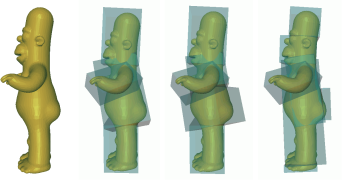
\includegraphics[width=0.5\textwidth]{img/related-work/mvbb.png}
	\caption{From \parencite{Huebner2008}: Minimum Volume Bounding Box on Homer model.}
	\label{fig:rel__mvbb}
\end{figure}

\begin{figure}
	\centering
	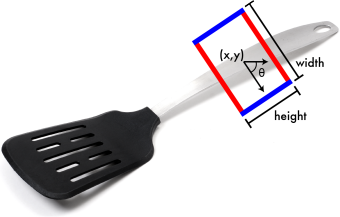
\includegraphics[width=0.3\textwidth]{img/related-work/grasp-representation.png}
	\caption{A five-dimensional grasp representation with terms of location, size and orientation. The blue lines demark the size and orientation of the gripper plates. The red lines show the approximate distance between the plates before the grasp is executed.}
	\label{fig:grasp-representation}
\end{figure}


\section{Machine-learned systems}
\label{sec:machine_learned_systems}
% rule based algorithms vs machine learning
Within artificial intelligence applications there are several approaches that can be used. A common design for these systems has been by using \emph{rule-based algorithms}. In this case there are a set of rules, most often crafted by humans, dictating the behavior of the system depending on certain conditions. Another approach is to use \emph{machined learned} systems. This second way of designing the system is based on having the machine learn from a set of observations. The learning process can be different, but revolves mostly around fitting a statistical model to the recorded observations as to be able to predict behavior in future observations.

\begin{figure}
	\centering
	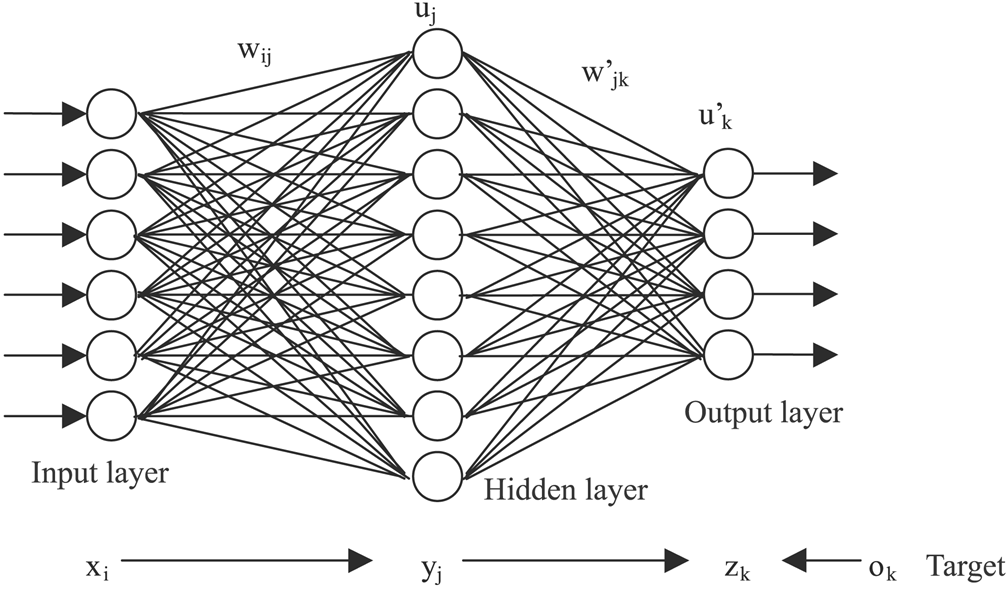
\includegraphics[width=\textwidth]{img/related-work/ann.png}
	\caption{Feed-forward layered artificial neural network [79]. Input layer communicates to
one or more hidden layers where the actual processing is done, computing the weights (w). The
hidden layers then connect to the output layer. Each hidden layer have a certain number of
artificial neurons, which have a defined activation function that produces the output for the
next neuron \parencite{extremetech}.}
	\label{fig:rel_ann}
\end{figure}

There are many different models that can be applied for machine-learned systems, and a very common one of them are \emph{Artificial Neural Networks} (ANNs). These models take inspiration from the way the human brain processes information. ANNs consist of a number (a network) of interconnected neurons which compute and propagate their output through a series of layers. An example showing the basic idea can be seen in figure \ref{fig:rel_ann}. The term \emph{Deep Learning} refers to ANNs that have a large number of layers.

Machine-learned systems have for a long time been very limited in their ability to process raw natural data. Careful and intelligent preprocessing has been required as to transform this raw data into a smaller set of features that is easier for the machine to learn upon. This includes noise reduction, feature selection and dimensionality reduction, and makes the preprocessing step no easy task as it requires an expertise knowledge of the domain that the system is to be used within and can be very time consuming to make sure it becomes correct. This is also linked to the high requirements in processing power that comes with working with high-dimensional raw data. However, with the advancements in hardware, ANNs and deep learning systems through their large multi-layer setup are able to learn a hierarchy of features and are making large progress within machine-learned systems to perform representation learning from raw data, minimizing the amount of preprocessing \parencite{Lecun2015}. In the example of computer vision, deep neural networks would learn how to extract global features such as edges from the image, and through the layers work on more complex features within the patches extracted from the previous layer.

Convolutional Neural Networks (CNNs) are a class of ANNs within deep learning that have a special architecture designed to process raw data that comes in multiple arrays such as the color channels in images which make them popular within computer vision. CNNs are structured as a series of stages where the firsts ones are usually composed of layers of type convolutional and pooling, with the goal to detect local conjunctions of features from the previous layer (\parencite{Lecun2015}, \parencite{Jarrett2009}). With minimal preprocessing CNNs can learn a variety of high- and low-level features to perform with great accuracy several tasks within visual recognition. \textcite{Lee2009} demonstrate through unsupervised learning of a convolutional network how the network learns in the early layers edge detection and object parts. \textcite{Turaga2010} show by emphasizing the learning stage, the CNN is able to learn edge detection with minimum pre- or postprocessing.

The performance of all types of ANNs is linked to their architecture. Changing the number of layers or their sizes can result in large fluctuations in performance, for the better or the worse. Some architectures become overtime more well-known for their success at certain tasks. One of them, named AlexNet, is the one published by \textcite{Krizhevsky2012} which achieved great results at the \textcite{ImageNet} image classification challenge LSVRC-2010. In their work they credit the performance of their neural network to its deep structure of many layers, showing that by only removing one of the convolutional layers its performance would decrease with about 2\%. Figure \ref{fig:alexnet_orig} illustrates the network architecture of AlexNet.

\begin{figure}
	\centering
	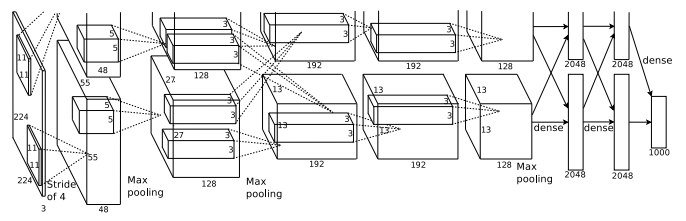
\includegraphics[width=\textwidth]{img/methods/alexnet_original.png}
	\caption{AlexNet architecture.}
	\label{fig:alexnet_orig}
\end{figure}

Machine-learned applications are becoming more and more frequently used because of their high performance, lower requirements for human intervention, as well with how it has become increasingly easy to collect and represent data in a more versatile way. The works in \parencite{Aleotti2012} \parencite{Suay2015} \parencite{Kim2004} all report good results for handovers between robots and humans, but are supported by rule-based algorithms. Rule-based algorithms can present some limits of adaptation to a wider spectrum of scenarios than those thought of when the algorithm was created. They can as well become error prone because of human factors. \parencite{Redmon2014} \parencite{Lenz2015} \parencite{Jiang2011} \parencite{Huebner2008a} are examples of work that instead use the advantages of machine-learned models to achieve good results, avoiding dictating the rules for grasping and handovers themselves. One disadvantage does nonetheless persist with these methods, which is the fact that their data sets for training require the time consuming task of manually labeling.


\section{Autonomous learning}


\subsection{Supervised and unsupervised learning}

Classification consists of creating a statistical model to determine the group (i.e. class) an observation belongs to. For machine-learned systems this requires them to find the connection between the features connected to an observation and their respective group. To achieve this we can use two different approaches: \emph{supervised} or \emph{unsupervised} learning.

Supervised learning uses a data set that is labeled, meaning that the observations within it are correctly assigned from the beginning. In this case we fit our model to the observations and their known label. On the contrary, in unsupervised learning any grouping of the observations is unknown to us. In this method we use cluster analysis to compute relationships between observations based on different metrics, and group them accordingly.

\emph{Autonomous learning}, also known as \emph{semi-supervised learning}, is a method of combining the two prior methods. Through unsupervised learning, groups are created for the observations and with a supervised learning algorithm a model is created to predict the group for future observations.


% learning from demonstration
\subsection{Learning by demonstration}

\begin{figure}
	\centering
	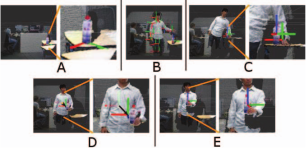
\includegraphics[width=\textwidth]{img/related-work/demonstrations.png}
	\caption{From \parencite{Chan2015a}: Stages of extracting grasp configurations from handover demonstrations. A - Object detection. B - Human detection and tracking. C - Grasp point detection. D - Direction of torso-to-hand vector for handover cue detection. E - Object orientation at handover.}
	\label{fig:rel__demonstration}
\end{figure}

\begin{figure}
	\centering
	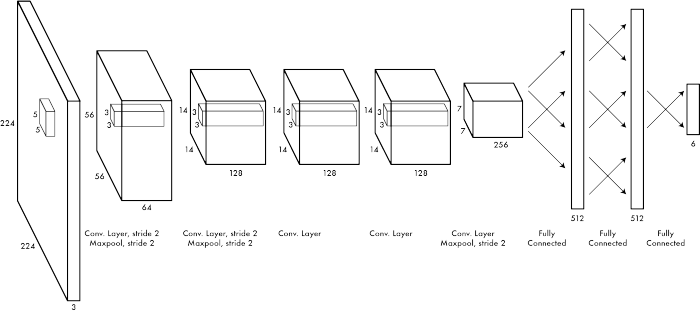
\includegraphics[width=\textwidth]{img/related-work/cnn-architecture.png}
	\caption{Full architecture used by \textcite{Redmon2014}.}
	\label{fig:rel__cnn-arch}
\end{figure}

A less explored research field is yet to teach robots grasping and handovers by demonstrations using vision. Having robots learn by observing humans would enable faster collection of data, save time from manually labeling and allow the robot to use more human-like motions. Common within robot simulation is that the data required for processing is represented by 3D models of the objects and environment (for example in \parencite{Miller2003}) which are not trivial to come by for newly encountered objects in a live setting as it would require the robot to see everything from all angles. Another factor is the accuracy of sensors and quality control of the data (i.e was it as good handover?) are some of the limitations of learning from observations which makes it a challenging method. Kinect sensors have become popular within robotics today because of their relatively low cost and support for depth data which can help in creating three dimensional renderings of images. \parencite{Lenz2015} \parencite{Redmon2014} \parencite{Jiang2011} \parencite{Saxena2008} are example of works that propose methods for training and identifying grasp sites using RGBD images recorded by a stereo camera, but the problem with these works is that they do not train on data collected by demonstrations without manual annotation. \textcite{Chan2014} collected data by observing humans interacting with objects, but the data covered other scenarios of object interaction than handovers. \textcite{Strabala2013} trained a model using decision trees from recorded data of humans performing handovers, but they had to manually label the recorded material with eye-gaze, two-dimensional position of participants, object locations and handover positions. \textcite{Chan2015a} do however propose a framework for robots to learn handovers and grasp sites through demonstration as seen in figure \ref{fig:rel__demonstration}. By handing objects to a robot they then have the robot repeat the handover in reverse order back to the human. They however do not have the robot learn any object features as to associate the handover settings to it, for the purpose of prediction.


% new objects
\subsection{Foreign objects}

One of the challenges within robotic grasping and handovers is the ability to perform their task on an object that the robot has never seen nor been trained for. Some previous research do enable grasping of foreign objects, but requires a lot of data which itself needs to be labeled. For example \textcite{Huebner2008a} in a continuation of their work in \parencite{Huebner2008}, train a neural network that can be used for grasping of novel objects, but requires the network to be trained on a previously manually labeled data set of grasps. Also the proposed model by \parencite{Chan2014} requires data on different ways to manipulate an object before the robot can calculate a way of grasping it and handing it over, making it hard to deploy in a new environment.

% how to use this related work for this thesis
\textcite{Redmon2014} show very promising results with their implementation in finding grasp sites on objects, even for those that are not present in the training set, illustrating the high performance of convolutional neural networks. Their work is based on the ImageNet model that was further trained with RGBD images for detecting grasp regions. The ImageNet model is however trained for RGB images, the authors solved this by dropping the blue channel and replacing it with the depth data. In figure \ref{fig:rel__cnn-arch} we can find an overview of the full architecture for their network. The problem is that the data that it needs for training is manually annotated. The framework proposed in \parencite{Chan2015a} is a good starting point for the collection of data as to train a model that can be later used for grasping and handovers. This thesis will try and combine these works by implementing a framework for collecting data through demonstration from humans and process it as to fit a convolutional neural network that can later predict grasping sites and handover features on foreign objects through RGBD images.


\chapter{Methodology}
\section{Overview}

The goal of this project is to develop a system that has autonomously learned from the handovers performed by humans to output an object's settings for how to be handed over, given an image of it. Another of our requirements is that the learning has been abstracted enough that this system is accurately applicable on new objects that are not present in the training set.

One way to go about with this would be by learning the handover settings for an object and then training for object classification. In other words, record all the handover features for each individual object, create a mean from them, and train a model to recognize the object based on images as to output its settings. Such a model would for \(n\) number of objects need to learn to output \(n\) different classes. This can potentially become an increasingly difficult task as the number of objects grows and with that the requirements on the size of the dataset grows, as to have the system be able to learn to properly recognize the objects. Such a system would believe that each object has its own unique settings, and might be not scalable to other objects absent from the training set.

If we instead hypothesize that some objects are handed over in similar fashion depending on their visual features we can try a different approach: letting the system by itself find relationships between the observations of handovers and through this classify the individual objects into their classes of handovers. After that the system is tasked with finding visual similarities between the objects that define which class they have been assigned. This simplifies our problem as the number of outputs shrinks. We no longer pressure the system into properly recognizing invidual objects, but instead similarities, which also lowers the requirements on data collection.

\begin{figure}
	\centering
	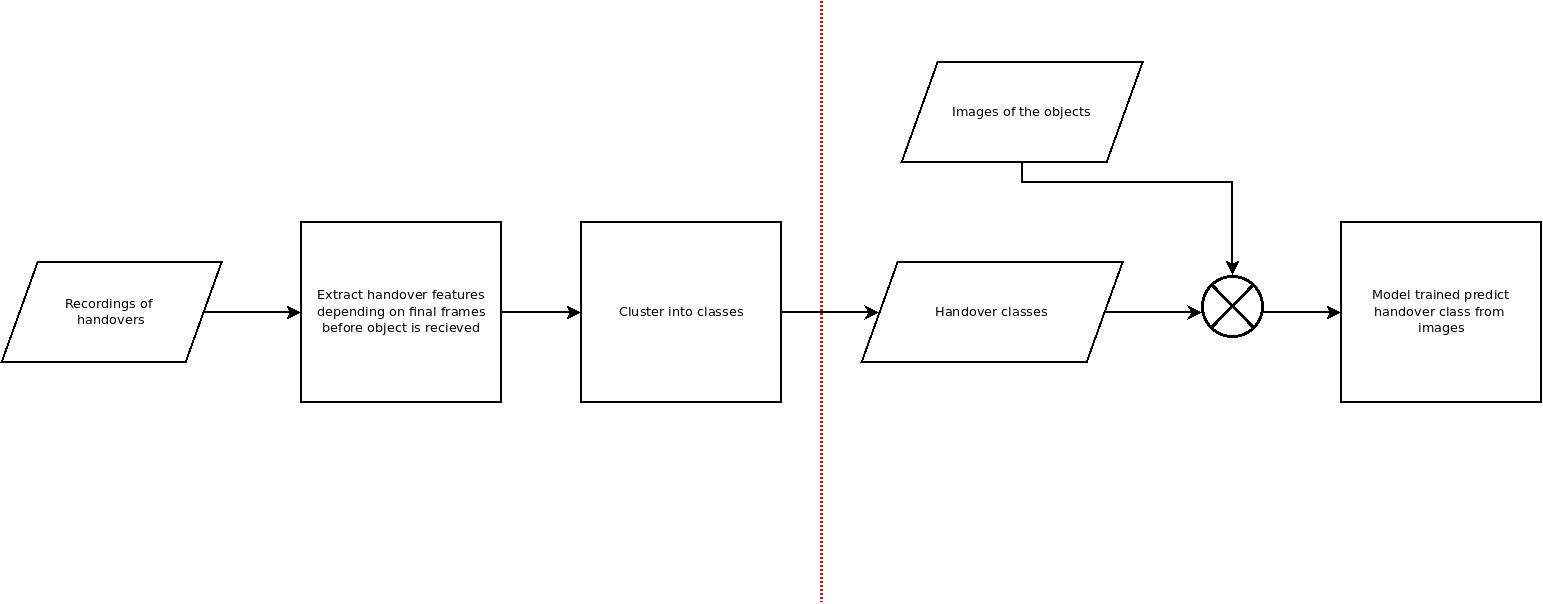
\includegraphics[width=\textwidth]{img/methods/flowchart.jpg}
	\caption{Flowchart describing the work process. Red delimiter marks the where the first part of the works goes over to the second part.}
	\label{fig:flowchart}
\end{figure}

In figure \ref{fig:flowchart} the workflow is summarized. The first part of this work will be to observe and record a number of handovers between humans for a defined set of objects which the system will try to categorise into different classes. In a second part each object will then be assigned a class that we train a machine to return when given an image the same object. Seeing how we do not have any labels for the handovers, but still want to train a model that outputs some defined class for how the object should be handed over, we will be using a semi-supervised approach in this project: by first applying an unsupervised learning algorithm to categorise and create classes of handovers that are later used as output for self-supervised learning.


\section{Tools and material}

\subsection*{Hardware}

During the project the following material were used:

\begin{description}
	\item[Kinect for Windows v2] Motion sensing device developed by Microsoft used for recording and taking pictures with support for color, depth and infrared data.

	\item[GeForce GTX 980 Ti] Nvidia brand GPU for better performance during training of for example deep neural networks that require a lot of data and processing power.

	\item[\textcite{AprilTags}] In order to extract data from the recorded frames about the objects we need to detect the objects themselves. Object detection is a very difficult part of computer vision and there are many different methods, where some are more robust than others, to do so. To help with this part to make data extraction easier and more precise we will be taking help of AprilTags. AprilTags can be compared to QR-codes that are printed out on small papers and fastened onto the objects. With the help of their software library we can easily track the objects in the recorded material by getting the position of the four corners of the tag, and its center, which enables us to estimate such things as pose of the object.

	\item[Fifteen different objects to be handed over] Chosen randomly around the house, all of which can be handed over using only one hand with ease. The set objects include: a knife, a screwdriver, a can, a box, a pair of cutters, a tube, a pitcher, a glass, a bottle, a brush, a cup, a hammer, a pen, a scalpel and a pair of scissors.

\end{description}

\begin{figure}
	\centering
	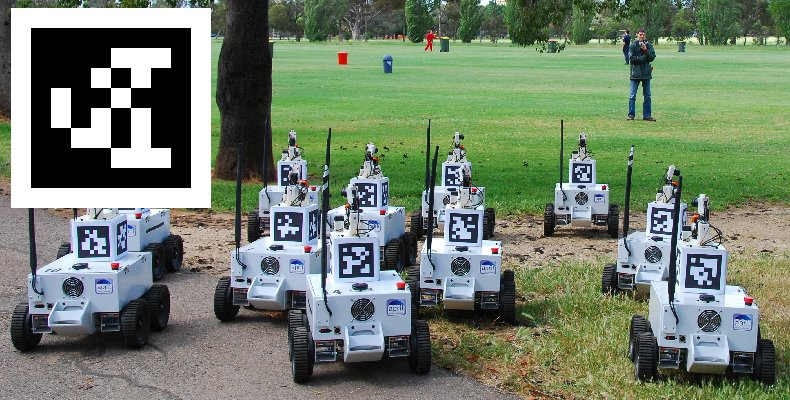
\includegraphics[width=\textwidth]{img/methods/apriltagrobots_overlay.jpg}
	\caption{Example of AprilTags in use on robots.}
\end{figure}

\subsection*{Software}

The applications will be written mostly in C++ or Python depending on availability of libraries. To help implement our system we will have the following programs and programming libraries at our disposal:

\begin{description}
	\item[\textcite{GIMP}] Image editing program that will be used for manual preprocessing of some images.

	\item[\textcite{libfreenect2}] Open source library written in C++ for communicating with the Kinect v2 camera.

	\item[\textcite{OpenCV}] Open source library for computer vision with bindings for C++ and Python, as well as other languages.

	\item[AprilTags programming library] C++ library written by the creators of AprilTag to help extract data from captured images such as the four corners of the tag and center of the tag.

	\item[\textcite{scikitlearn}] Python machine-learning library. Contains several useful tools for implementing and training models, as well as data processing.

	\item[\textcite{Tensorflow}] Open source Python library for creating and training neural networks with GPU support for more efficient processing time.

\end{description}


\section{Categorisation of handovers}

\subsection{Recording of handovers}

For this purpose a number of voluteers were asked to be recorded while handing over a set of objects between each other. Even though Kinect v2 supports depth images, only two-dimensional color data will be used in this part. A total of 11 people who already knew each other from before volunteered (including myself) for this task. Pairs of volunteers were permuted as to try and make each person while being the giver adapt to different receivers. Instructions for handing over the objects were given prior to recordings as to make sure participants gave the object in a manner that the person receiving the object can use it straight away after grasping it. For example the hammer should be handed over with its handle first in a manner that the next person can start hammering directly without requiring a switch of grip after receiving it. Or a cup is to be handed handle-first so the person can start drinking right away. A bottle is easier to pour from if you hold it below its center of gravity therefore this area should be free for the receiving person while handing it over. For reasons that we will see later participants were instructed to use a grasp that covers the object, they could not for example hand something over flat in their palm. This is because of how the grasp region is identified and its limitations. The general regions of where to grasp by the giver and what part to present to the person receiving were chosen by myself with in mind for optimization for the receiver when given the object. For objects that might contain liquids the participants were asked to imagine that these objects were filled to the top while handing them over between each other.

\subsection{Extracting features}

% TODO write more about image moments
% TODO write about homography

\subsubsection{Orientation of the object}

The first set of features that we will extract from the recorded material will be around the orientation of the object when being handed over, i.e. the transformation from its ground truth to the observed position. Before any work is done with the recorded material, for each object we manually create a reference image representing its ground truth position. The orientation of the ground truth was chosen to be the object's orientation while in common resting position (e.g for a bottle, standing up). For those objects that are layed down, their orientation was chosen to be with their head upwards. From these images we also generate binary masks that will be used to mask out the object after detection. Figure \ref{fig:objects_montage} shows the reference images created and figure \ref{fig:masks_montage} shows their binary masks. These images were created using the image manipulation software GIMP.

\begin{figure}
	\centering
	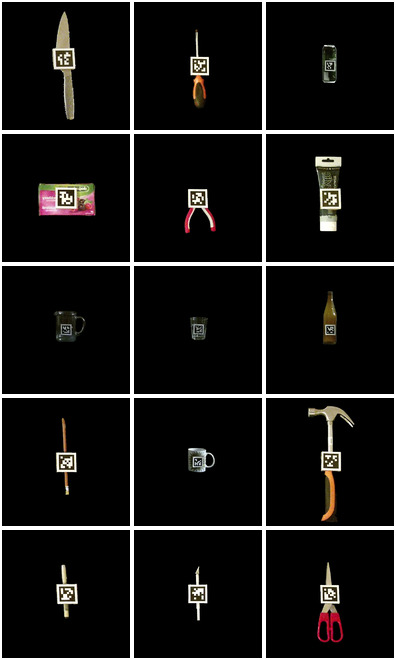
\includegraphics[width=\textwidth]{img/methods/objects.jpg}
	\caption{Ground truth images of the objects used with an AprilTag fastened to them.}
	\label{fig:objects_montage}
\end{figure}

\begin{figure}
	\centering
	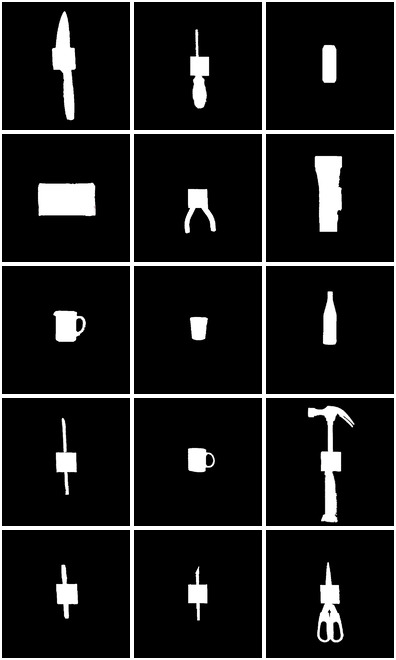
\includegraphics[width=\textwidth]{img/methods/masks.jpg}
	\caption{Binary mask of each object}
	\label{fig:masks_montage}
\end{figure}

One of our biggest challenges with the project is to actually detect the object in each frame. This is a very non-trivial task and there is much research around methods for object detection. To help us with this part of the project and make esure that the data we extract is accurate, we will use AprilTags. They can easily identify the four corners of the tags in a frame and by this way locate the object. Using the OpenCV library and their \texttt{findHomography} function, we can compute the homography matrix that transforms the four corners of the tag in the reference image to the corners of the tag found in the frame. A homography matrix \(H\) is a 3x3 matrix with a total of nine values which creates quite a few features if we would try and cluster on it. Also it contains data on how to translate the object in three-dimensional space, which in our case is irrelevant as we are only interested in a way of defining the orientation of the object and are only working with two-dimensional data.

Alternatively we can calculate a rotation of the object and through an angle represent its orientation with instead only one feature. As we are only working with two-dimensional data we will only interest ourselves for the rotation on the z-axis. From the homography we can calculate a rotation matrix from which we can later derive the searched angle. Using the Python code presented in \ref{lst:rotation_matrix} based on the OpenCV library, we compute a 3x3 rotation matrix \(R\). Using the rotation matrix we can compute the angle \(\theta_R\) as \(\theta_R = \arctan(R_{1,0} / R_{0,0})\). In this case the rotation will be around the center of the tag because it is from which we calculated the homography matrix.

The previous homography matrix can though still be used to transform the binary mask of the object, and then be applied on the frame as to mask out only the object. From this we can afterwards retrieve a grasp region of the object.

\begin{lstlisting}[
	language=Python,
	frame=single,
	label={lst:rotation_matrix},
	caption={Python code to calculate rotation matrix from homography matrix using OpenCV and numpy libraries (taken from \parencite{OpenCVHomographyDemo}).},
	float,
	floatplacement=H,
	]
norm = np.sqrt(np.sum(H[:,0] ** 2))
H /= norm
c1 = H[:, 0]
c2 = H[:, 1]
c3 = np.cross(c1, c2)

R = np.zeros((3, 3), dtype=np.float64)
for i in range(3):
	R[i, :] = [c1[i], c2[i], c3[i]]
w, u, t = cv2.SVDecomp(R)
return np.dot(u, t)
\end{lstlisting}

\subsubsection{Grasp features}

Skin color is a quick way of segmentating and finding grasp region as the color of skin is quite different from the colors of the objects, but the method is not too robust in covering many different people as the color can vary quite a lot from person to person. The setting for skin color had to therefore be tweaked manually depending on the participant. By using the homography matrix and the binary image, we have been able to mask out the object from the scene. This image of the found object is later segmentated by skin color. A contour expressed as a rotated rectangle is then calculated around the largest segmentated region found, which represents our grasping region.

A rotated rectangle is composed of three different parameters: width, height and angle. Another possible feature we can extract is the ratio between area of grasp region and area of object. Using the binary image of the object we can compute its area \(A_{object}\) with the help of OpenCV by using \texttt{findContours} and \texttt{contourArea}. The area of the rotated angle is simply \(A_{grasp} = width \times height\) and the ratio between them becomes \(A_{ratio} = \frac{A_{grasp}}{A_{object}} \).

The last features that we can extract are: the distance \(\Delta\) as the L2 norm between centers of the grasp region \(O_{grasp}\) and center of mass of the object \(O_{object}\), and the direction between these centers. The center of mass can be computed using the image's moments of the binary image. Moments are retrieved with the help of the \texttt{moments} function, part of the OpenCV library, then the following formula gives us the center:

\[
	O_{object} = \frac{M_y}{M}, \frac{M_x}{M}
\]

We can then extract the distance between center of mass of the object and the center of the grasping region as a feature. It also enables us to create a unit vector from the center of mass of the object towards the grasping region.

% TODO write better later
To summarize we can extract the following features:
\begin{itemize}
	\item Rotation of object in z-axis, extracted from the homography matrix of the AprilTag.
	\item Distance between center of mass of the object and the center of the grasping region.
	\item Ratio of distance between center of mass of the object and the center of grasp, over the diagonal of the object.
	\item Direction in x-axis between center of mass of the object and the center of the grasp.
	\item Direction in y-axis between center of mass of the object and the center of the grasp.
	\item Ratio of area of the grasping region by the area of object.
	\item Width of grasp region.
	\item Height of grasp region.
	\item Angle of grasp region.
	\item Center of grasp region.
	\item Center of mass of the object.
\end{itemize}

With these features we define for a robot how to grasp an object and present it to a human for a handover. This list of features is however quite large and represents a very high-dimensional set of data. High-dimensionality can become quite problematic as the values might not vary with the same amount in all dimensions as well as create similarities between objects that are not there. A first filtering of these features can be made on the idea that the features should be expressable invariant to the object, i.e. we only keep the features that are expressed in relation to the object. This will leave us with the following list:

\begin{itemize}
	\item Rotation of the object in z-axis, expressed between 0.0-1.0 where 1.0 is a full circle (360 degrees).
	\item Direction in x-axis between center of object and center of grasp.
	\item Direction in y-axis between center of object and center of grasp.
	\item Ratio of distance between center of the object and the center of the grasping region.
	\item Ratio area of grasp region over area of object.
\end{itemize}


\subsubsection{Filtering of unwanted frames}

One recording session consists of one pair of volunteers during which the one giving has handed over all objects in the set to the receiver. In this project we only interest ourselves for the features that define how an object is to be presented to the one receiving it, i.e. the actual moment in the end of the handover motion when the giver holds out the object ready for the receiver to take it. At all times of this session the application is continuously recording, creating a large number of frames that are of no interest such as when the participant handing over the objects is fetching the next one or the person receiving is putting one of them away. Some preprocessing of the frames is therefore required to find the frames of interest.

A first step is to create a Region of Interest (ROI) in which we will concentrate on searching for objects. This will not only help filter out the vast amount of frames that are not of interest, it will also help with performance as opposed to if we were searching the entire frame. Our ROI is arbitrarely set to the middle of the frame where the person handing over the object would finish the movement, and set to be large enough to detect the tag and see the entire object. When a tag is detected within the ROI we flag this frame to be a handover moment before extracting the features. This is unfortunately not enough because we might be flagging frames where the receiver is holding the object after taking it, or maybe both are holding it but the system detects the receiver's hand as the largest grasping region. Figures \ref{fig:handover_bottle} and \ref{fig:handover_hammer} demonstrate frames that the system detected as handovers with the objects masked out and the grasping region identified. The methods explained above might also be incorrect as the grasping region was incorrectly detected. Manual filtering was later applied to images that were flagged as handover moments and to make sure they were correct ones and that the data extracted was correct. Figure \ref{fig:handover_incorr} illustrates a situation that needs to be manually filtered out when the system percieves to have identified a handover situation but the grasping region identified is that of the receiver's.

\begin{figure}
	\centering
	\begin{subfigure}[t]{\textwidth}
		\centering
		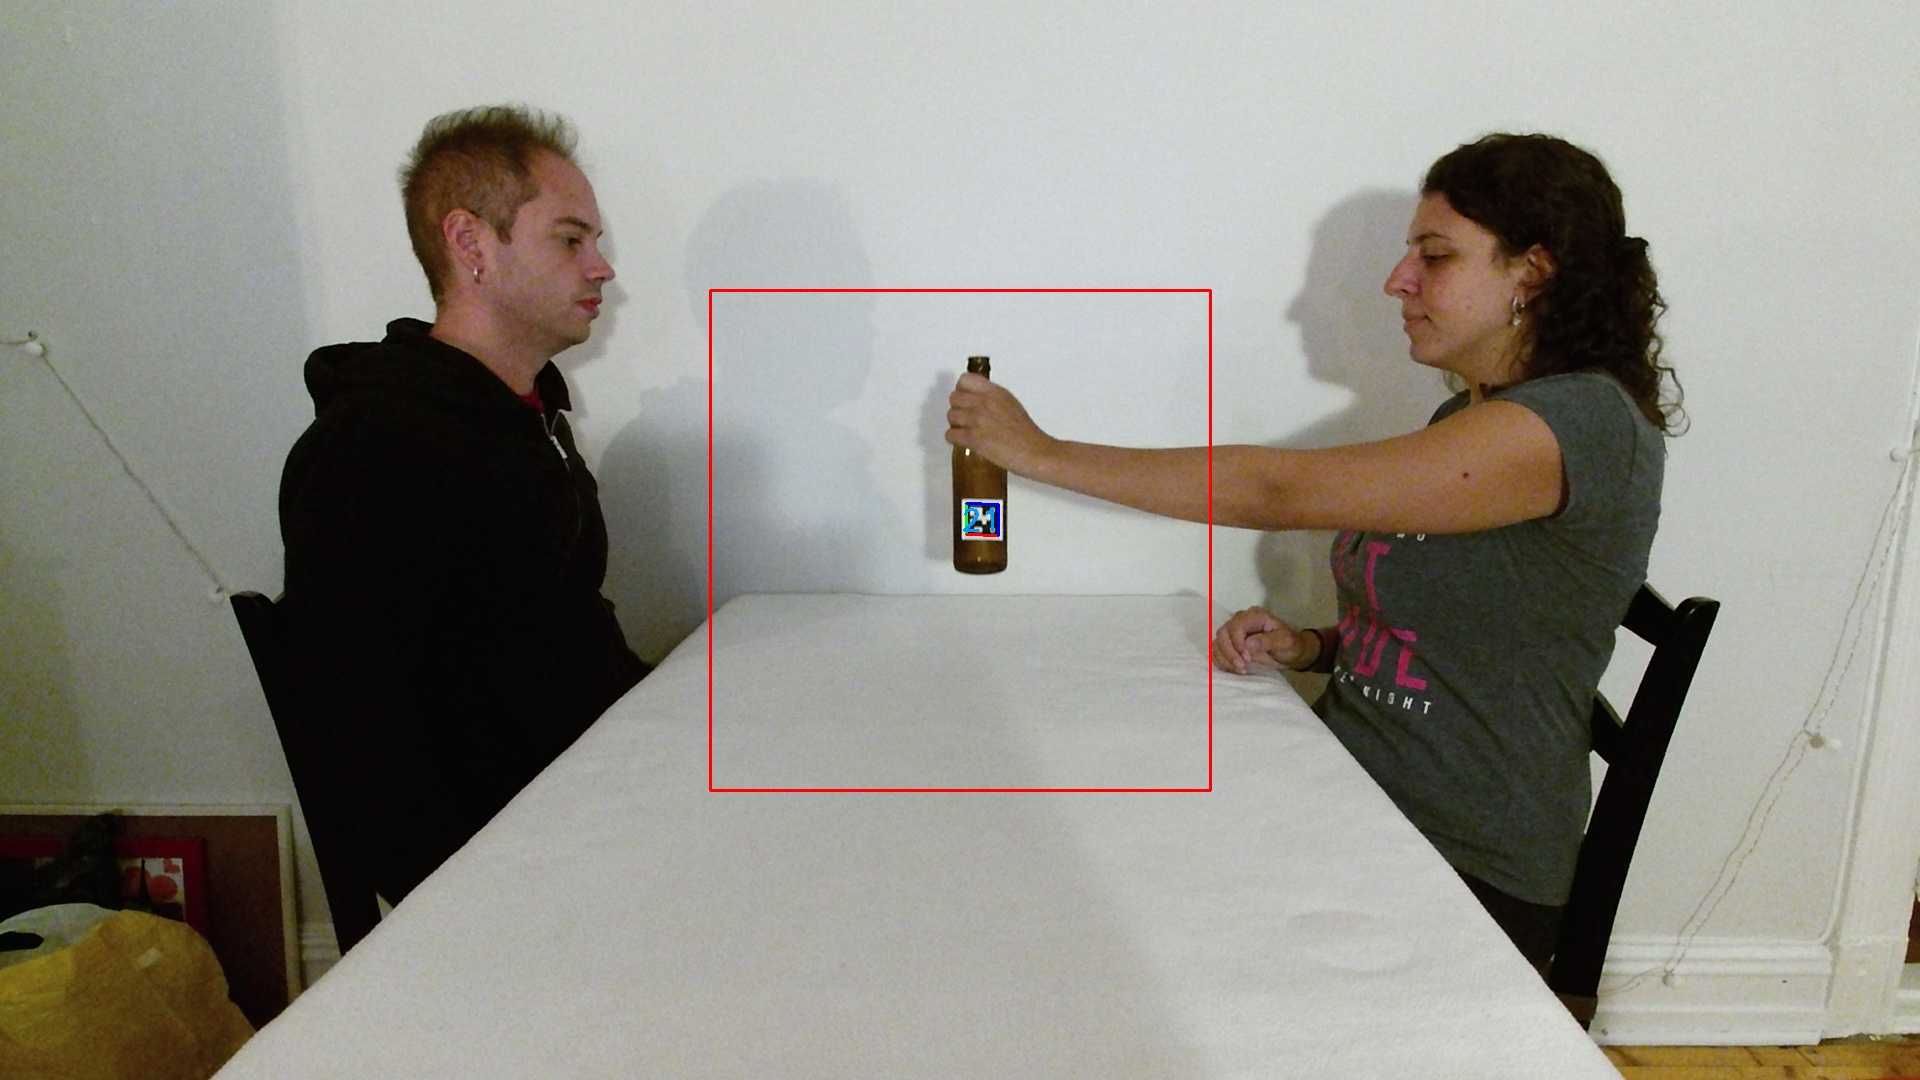
\includegraphics[width=\textwidth]{img/methods/handovers/bottle_frame.jpg}
		\caption{Handover of bottle.}
		\label{fig:demo_handover_bottle}
	\end{subfigure}
	\par\bigskip
	\begin{subfigure}[t]{0.5\textwidth}
		\centering
		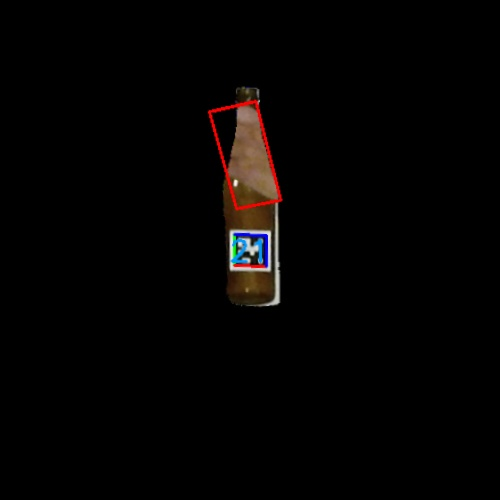
\includegraphics[width=\textwidth]{img/methods/handovers/bottle_masked.jpg}
		\caption{Bottle masked out and grasp region identified.}
		\label{fig:handover_bottle_masked}
	\end{subfigure}
	\caption{Handover demonstation of a bottle with the grasp region detected after being masked out. The giver was instructed to pretend like the bottle was full of liquids to make sure they held it upright.}
	\label{fig:handover_bottle}
\end{figure}

\begin{figure}
	\centering
	\begin{subfigure}[b]{\textwidth}
		\centering
		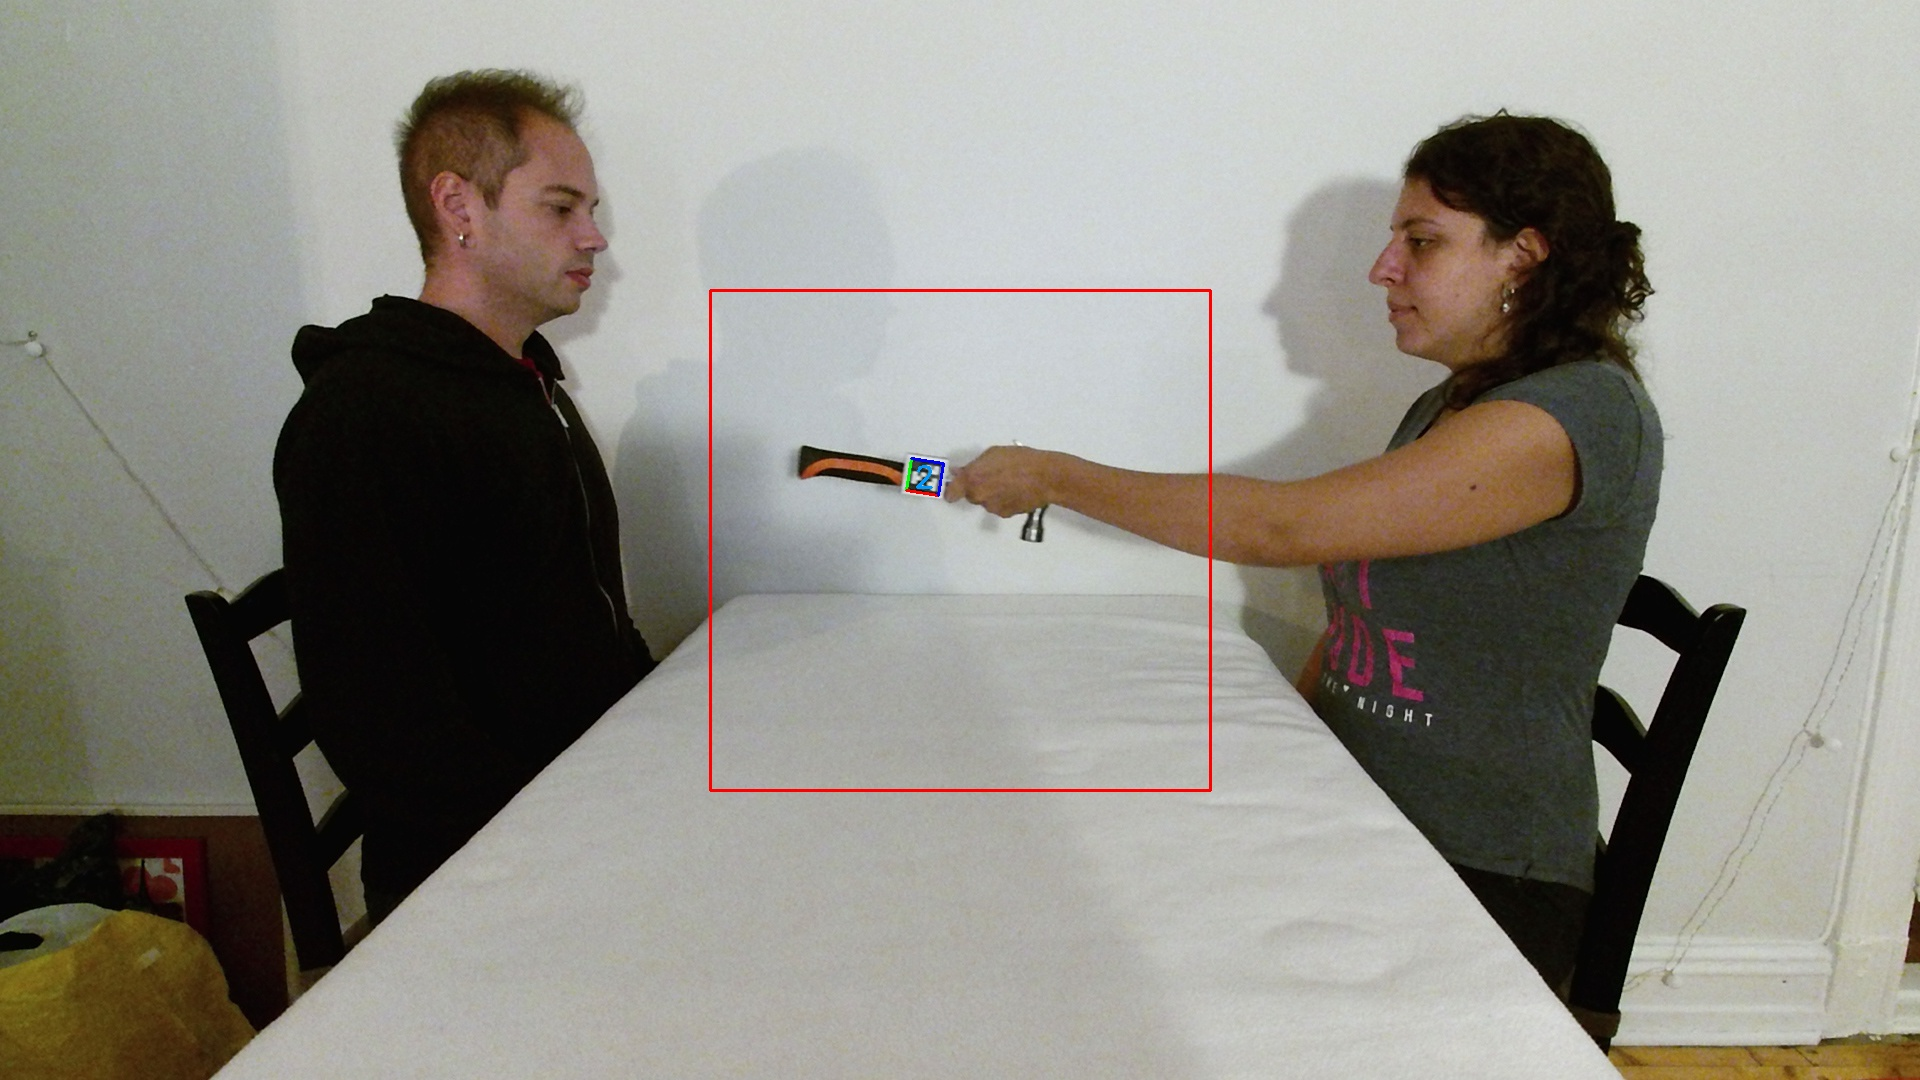
\includegraphics[width=\textwidth]{img/methods/handovers/hammer_frame.jpg}
		\caption{Handover of hammer}
		\label{fig:demo_handover_hammer}
	\end{subfigure}
	\par\bigskip
	\begin{subfigure}[b]{0.5\textwidth}
		\centering
		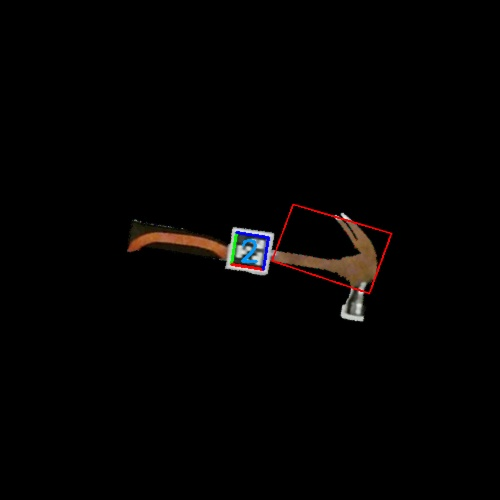
\includegraphics[width=\textwidth]{img/methods/handovers/hammer_masked.jpg}
		\caption{Hammer masked out and grasp region identified.}
		\label{fig:handover_hammer_masked}
	\end{subfigure}
	\caption{Handover demonstration of a hammer with the grasp region detected after being masked out. The giver was instructed to give it handle first, holding the head so the receiver is able to use it straight away.}
	\label{fig:handover_hammer}
\end{figure}

\begin{figure}
	\centering
	\begin{subfigure}[b]{\textwidth}
		\centering
		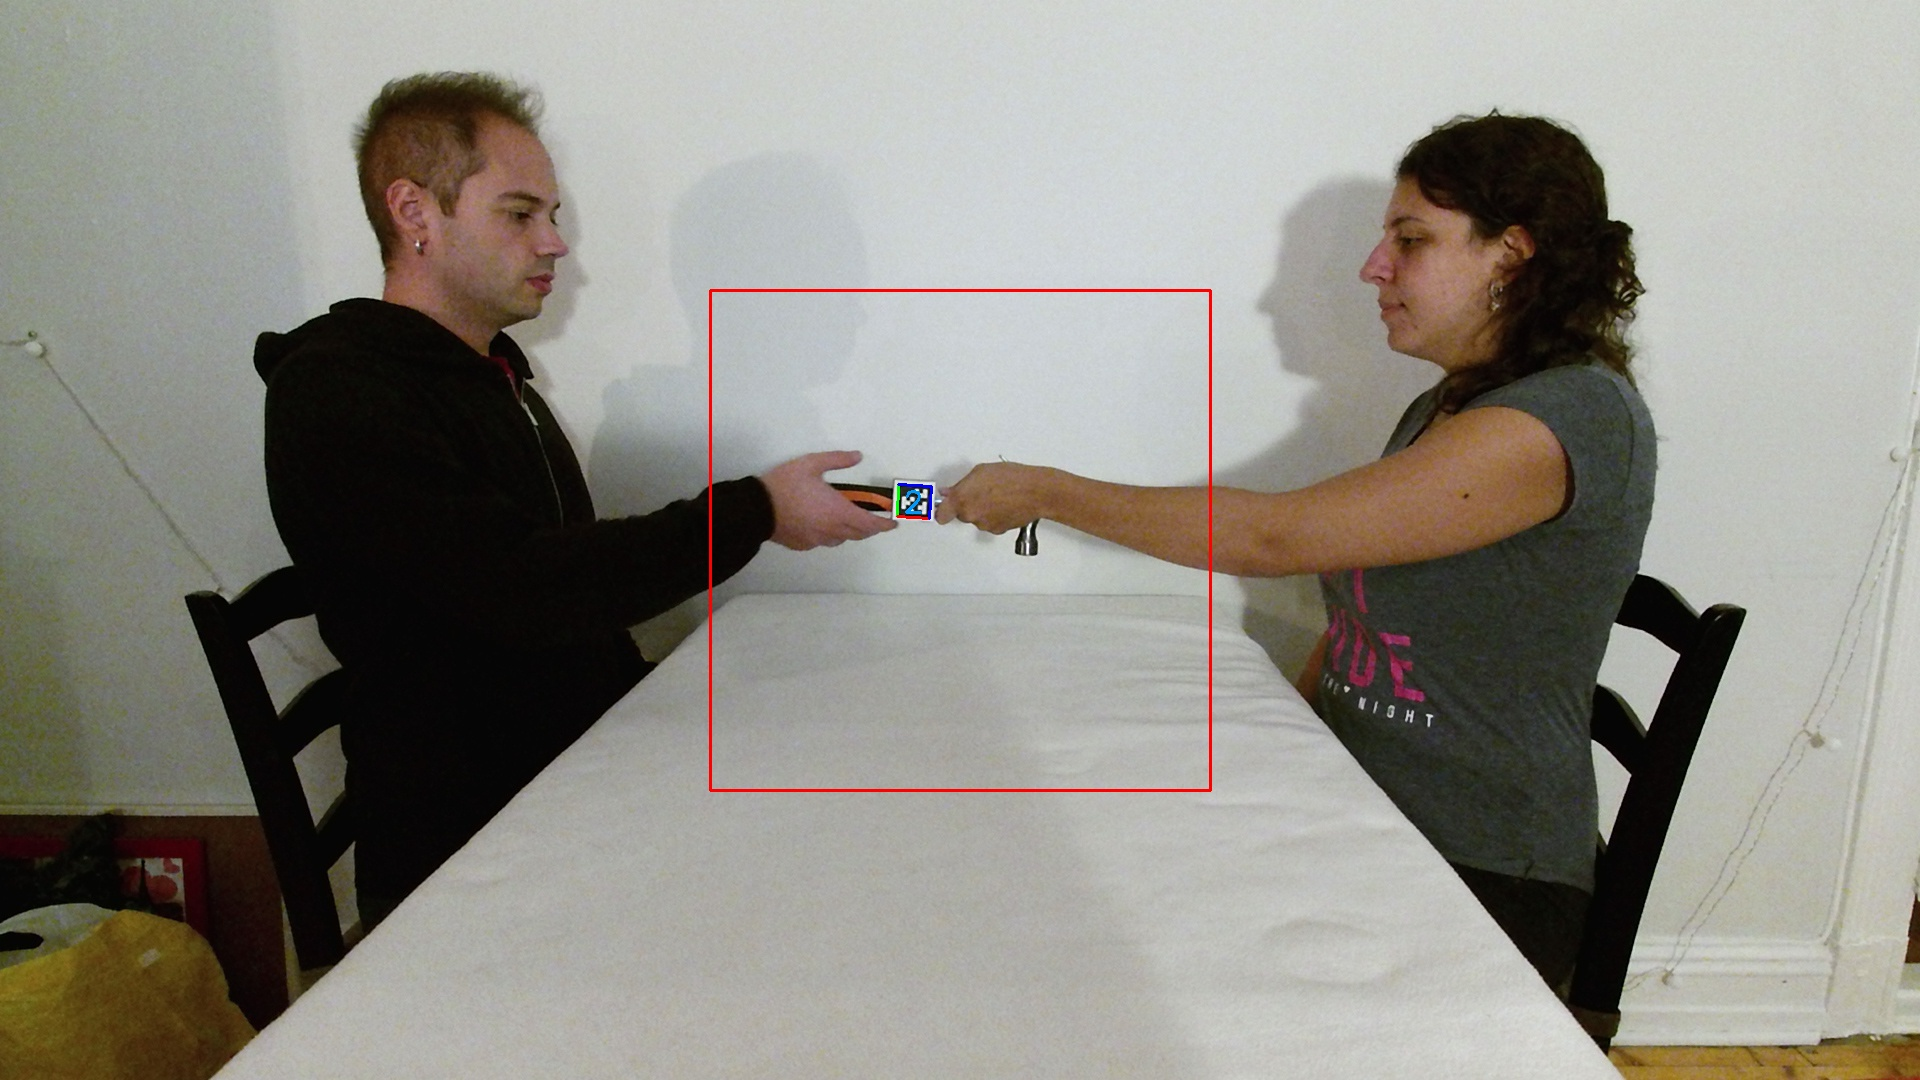
\includegraphics[width=\textwidth]{img/methods/handovers/incorr_frame.jpg}
		\caption{Handover of the hammer after the receiver takes the object.}
		\label{fig:demo_handover_incorr}
	\end{subfigure}
	\par\bigskip
	\begin{subfigure}[b]{0.5\textwidth}
		\centering
		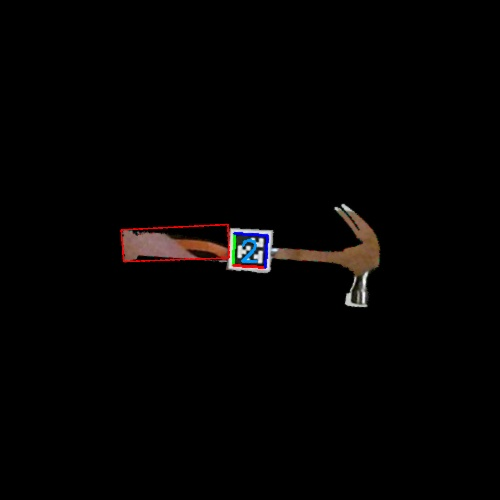
\includegraphics[width=\textwidth]{img/methods/handovers/incorr_mask.jpg}
		\caption{Hammer with the grasp region of the receiver identified.}
		\label{fig:handover_incorr_masked}
	\end{subfigure}
	\caption{Example of frame with false positive. The object is detected within the region of interest but the identified grasping region is not that of the giver, but the receiver's.}
	\label{fig:handover_incorr}
\end{figure}


\subsection{Clustering by handover features}

After observing a number of handovers betweens humans, a first step is to try and categorise these handovers into different classes that can be applied for the objects. As we do not have any labels, or even unsure how many different categories of handovers we have recorded, we will attempt at clustering using an unsupervised learning algorithm by the features that we have extracted from the recorded material.

\subsubsection{K-Means} % TODO references

For the purpose of categorizing the handover samples we will be using the \emph{k-means} algorithm. K-means is an algorithm that attempts to classify a number of observations into \emph{k} number of clusters. The algorithm starts by creating \emph{k} number of centroids for each cluster and assigning our samples to the centroid within shortest distance. The algorithm iteratively then updates the centroids to become the mean of the samples assigned to it, and then re-assigns all samples depending on the new centroids. This is repeated either a fixed number of times or until the algorithm converges minimizing the sum of squares within the clusters.

We are faced with the problem that we do not know in advance how many clusters are best suited in this case. We will run k-means for a range of different number of clusters between two and fifteen, thereafter we will use the \texttt{elbow method} and the mean \texttt{silhouette coefficient} to decide what is the best fit.

The more clusters you have the better it would fit your data. Imagine that you had the same number of centroids as samples, you will in this case have a perfect fit because all samples would have a distance to the centroid of zero. On the other hand what we really are searching for is the \texttt{fewest} number of clusters that gives the best "reasonable" fit. While starting with a small number of clusters and then gradually increasing the number step by step, by observing the plot the sum of distances between the samples and their assigned centroid gradually descreases. When the gradient from one observation to the next is below a certain threshold, we deem the observation as good fit. This is referred to as the \texttt{elbow method}.

The formula for the \texttt{silhouette coefficient} of a sample is as following:

\[
	\frac{(b - a)}{max(a, b)}
\]
\[
	a = \text{distance from sample to assigned centroid},
\]
\[
	b = \text{distance from sample to nearest centroid other than assigned one}
\]

Silhouette coefficients range from 1 to -1. 1 is the best score because ideally the distance to the centroid is close to zero (\(a = 0\)) which would give us \(b / b = 1\). A score of zero indicates that some clusters might overlap each other, and a negative value shows a sample that has been assigned the wrong cluster. By looking at the mean silhouette coefficient of all samples, we can choose the number of clusters that maximizes the mean value.

Neither the elbow method nor the mean silhouette coefficient are not enough by themselves to make an accurate decision on the number of clusters, but together they give us a very good estimate. We will therefore start by looking at the mean squared distances of the samples to their centroids and using the elbow method to define a possible interval of possible values for number of clusters, and last use the mean silhouette coefficient to conclude.



\subsubsection{Principle component analysis (PCA)}

A challenge that presents itself using clustering algorithms is choosing what features are to be used for the purpose. All features are not equally important into classifying the samples. \textcite{Ding2004} showed in their work through principal components and K-means, the relevance between unsupervised dimension reduction and unsupervised learning. We will be using \emph{Principle component analysis} (PCA) to evaluate which features that are to be used to define each cluster. Ideally we use the smallest number of features possible, but also the ones that create the most distinct clusters. PCA defines the principal features as those with the highest variance. It reduces the dimensionality by calculating the variance over all dimensions, i.e. features, and either choses a fixed number of the highest ones or keeps those that represent a certain ratio of the total variance within the data.

%
% Prediction of handover class
%


\section{Prediction of handover class}

As mentioned our aim in the end is to have a robot be able to predict a handover setting given an image of an object. In our case we will have it predict a class of handovers which are the result of the previous clustering. The system needs in this case to be able to relate visual features that come through imagery, to the class, also in a sufficiently abstract way that it can accurately predict the class for an unencountered object during training.

\subsection{Convolutional Neural Networks}

We hypothesize in this case that there is a number of features that can be retrieved visually from the objects, that define which class of handovers it belongs to. Even though we could try and preprocess all sets of objects and re-define them as a set of features, such as decomposing them into geometrical shapes, choosing which features it should be and how to retrieve them would be a challenging task, especially before knowing the results of the clustering. In \ref{sec:machine_learned_systems} we mentioned convolutional neural networks and works such as \parencite{Lee2009}, \parencite{Turaga2010} where the layers through training are able to hierarchically extract features in the images to later perform precise visual tasks. This ability of CNNs corresponds well with our goal to have the machine learn atonomously without human preprocessing or labeling. Through training on a dataset of images, our hope is that the machine will be able to draw relations between visual features extracted from the images with a certain class of handovers.

\subsection{AlexNet network}

For the task of predicting handover class from an image we will be training a convolutional neural network. The most challenging part with all artificial neural networks is to define their architecture. Changes to the number of layers and their sizes can play a significant role on the outcome of the results. Within object classification there have been a number of architectures proposed that have achieved good results, one of these is the \texttt{AlexNet} network which was mentioned in \ref{sec:machine_learned_systems}, and we will use as basis for our own network.

The AlexNet was designed for the ImageNet object classification problem in 2010, trained over 1,2 million images to output 1000 different classes. As a reminder, figure \ref{fig:alexnet_orig} shows the network architecture used by the AlexNet. It includes in total eight layers, all of which use ReLU non-linearity as activation function:

\begin{description}

	\item[Five convolutional layers] The first convolutional layer filters the \(224 \times 224 \times 3\) input image with 96 kernels of size \(11 \times 11 \times 3\) with a stride of 4 pixels. The second convolutional layer takes as input the (response-normalized and pooled) output of the first convolutional layer and filters it with 256 kernels of size \(5 \times 5 \times 48\). The third, fourth, and fifth convolutional layers are connected to one another without any intervening pooling or normalization layers. The third convolutional layer has 384 kernels of size \(3 \times 3 \times 256\) connected to the (normalized, pooled) outputs of the second convolutional layer. The fourth convolutional layer has 384 kernels of size \(3 \times 3 \times 192\) , and the fifth convolutional layer has 256 kernels of size \(3 \times 3 \times 192\).

	\item[Three fully connected layers] with 4096 neurons each, where the last one is fed to a 1000-way softmax output.

\end{description}

In total the network consists of 60 million parameters and 650 000 neurons. At the time, the designers of the network were under the restriction of the performance of GPUs, hence the parallell system. Seeing how our classification problem is of significantly smaller scale its size will do without problem, note however that we will re-design it so it runs sequentially on one GPU. The only other modification we will attempt will be by adding a new fully connected layer at the end with size depending on the results from the prior clustering. Figure \ref{fig:method_cnn_arch} shows our network architecture. As a side note: since the AlexNet network was designed, several other successful network architectures have been proposed, some that even outperform AlexNet. Such as \texttt{VGG-16} by \textcite{Arge2015} and \texttt{Inception} by \textcite{Szegedy2014}. These networks are however larger and deeper which would in theory require more processing time and as well as more data to train, both which are of limited supply. The AlexNet therefore makes a good compromise and should still be well suited for our smaller problem.

\begin{figure}
	\centering
	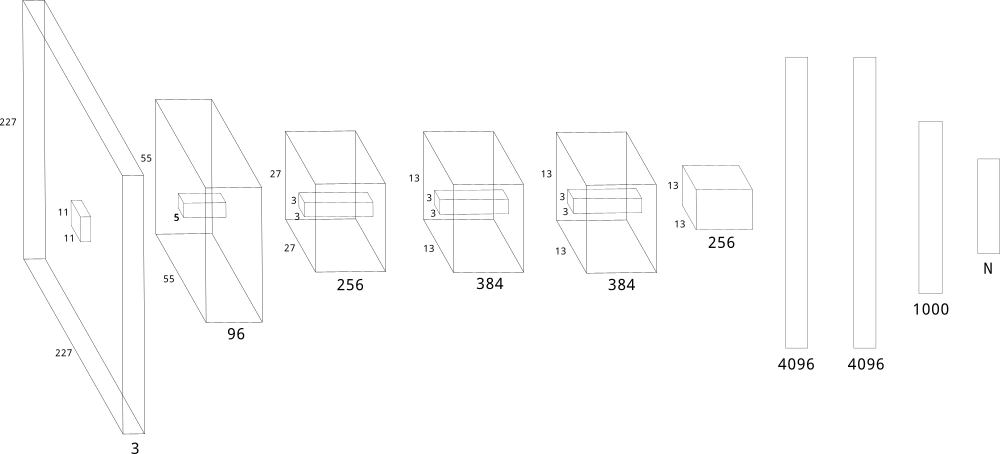
\includegraphics[width=\textwidth]{img/methods/network.png}
	\caption{Final version of the architecture. Serial version of the AlexNet architecture with an extra fully connected layer that has the same N number of outputs as the results from the clustering.}
	\label{fig:method_cnn_arch}
\end{figure}

\subsection{Training and testing}

We want the machine to learn from the handovers between humans that it has observed. We will therefore only use as our dataset the objects that were used for recording handovers. Despite their potential for performing very well, one issue with ANNs (especially very deep ones) is that they often require a lot of data to do so. The amount of data we are able to gather by taking images of the objects is unfortunately not enough for a network as large as the AlexNet network which was designed for over a million images. Fortunately for us there are pre-trained weights to be found that we can work upon and increase our chances of success. At \parencite{AlexNetImplWeights} we can find a set of pre-trained weights to use and also we can find a good base for our own implementation of the architecture using the Python library \texttt{tensorflow}.  Next step is to finetune the pre-trained weights to better fit our own data and fit it to our desired output.

Color images contain three channels of color (RGB) to define their texture. We theorize that it is not only the texture that defines the visual features of a handover class but also the shape of the object. Three channels of color can therefore feel redundant if the color is not the only thing that defines what the objects have in common. It can also create distinctions between the objects that are unnecessary and maybe confusing for the network to learn as it will make it harder to learn relations between them. Depth data gives a good 2,5-dimensional representation of the shape of the object, which can also be visualized by converting it to a grayscale image. This can be seen as one channel of color. As input data we will be taking inspiration from \parencite{Redmon2014} and perform the same alterations to our own dataset by replacing the blue color channel with the depth image. Figure \ref{fig:rgbd} shows an example of the hammer with its RGB image to the left, depth image in the middle and to the right the color image with the blue channel replaced for the depth data. Using the Kinect v2 camera, both color and depth images were taken of all objects from several different angles in different positions. Data augmentation was later performed on the resulting images to enlargen the dataset by using flipping, random cropping and random rotations of the images.

There are issues like black triangles in the corners or along the edges after rotating and/or cropping. These images are unwanted as the network might identify these regions with the objects. Therefore all the images created through data augmentation will be gone through manually as to make sure they are all suitable for training by the network. After we are done selecting images for our dataset we are not guaranteed that it is balanced between the objects or the classes. To prevent any overfitting we will also make sure that we balance the dataset evenly over all objects and classes.

\begin{figure}
	\centering
	\begin{subfigure}[b]{0.3\textwidth}
		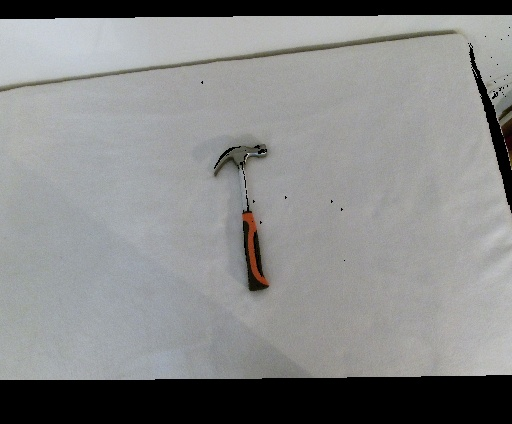
\includegraphics[width=\textwidth]{img/methods/rgbd/rgb.jpg}
	\end{subfigure}
	\begin{subfigure}[b]{0.3\textwidth}
		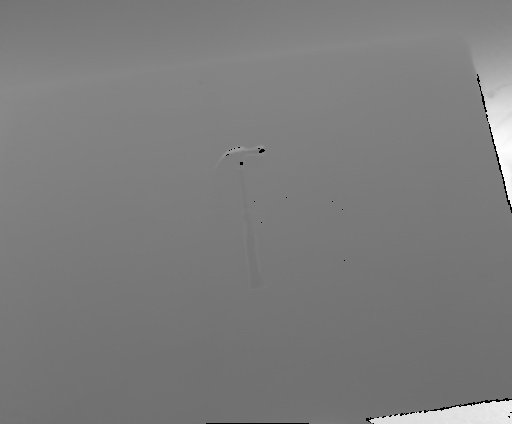
\includegraphics[width=\textwidth]{img/methods/rgbd/depth.jpg}
	\end{subfigure}
	\begin{subfigure}[b]{0.3\textwidth}
		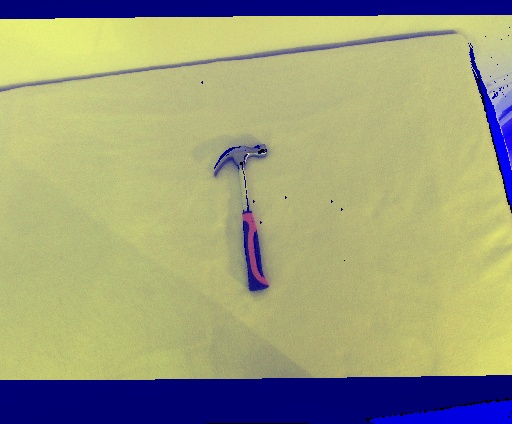
\includegraphics[width=\textwidth]{img/methods/rgbd/rgbd.jpg}
	\end{subfigure}
	\caption{RGB-, depth- and RGB-image with blue channel replaced by the depth data for the hammer.}
	\label{fig:rgbd}
\end{figure}


\section{Testing}
\label{sec:testing}

The training and validation of the model will be done on images from the objects that were used for training. This is to validate how well the model performs on objects that it has been trained for.

For testing purposes a number of images will be taken of objects that are not part of the training set. This is to see how well the model abstracts to other objects than the ones that it was trained on. On the contrary to the objects used for training we will not record handovers for these. Instead we will manually decide which class they belong to. This means that we are required to choose objects that in some ways resemble the objects from the training set and that have a quite decisive way of being handed over, so it does not become too questionable about which class they belong to. These objects are chosen depending on the results achieved from the clustering, further explanations are presented in section \ref{sec:res_setup}. The list of objects used for testing is as follows:

\begin{itemize}
	\item Beer glass.
	\item Bottle, a larger one than the one trained on.
	\item Carafe.
	\item Cup, different from the one trained on.
	\item Fork.
	\item Glass, with different shape from the training set.
	\item Knife, smaller and different shape than the one trained on.
	\item Scissors, smaller than the one trained on.
	\item Spatula.
	\item Spoon.
	\item Wine glass.
	\item Wooden spoon.
\end{itemize}

The images of the objects will be inputed to the model and the accuracy will be tested against it. As there are no other methods to measure against we set as an aim of this project to reach an accuracy of 90\% with a standard deviation of 5\%. If these results are achieved we judge the model to be successful.


\chapter{Results and discussion}
% ======================================================================================
% CLUSTERING
%
% graphs to insert:
%	- score vs silhouette coefficient per cluster
%	- sample silhouette values for the best number of clusters
%	- 3D/2D cluster representation for the best number of clusters
% tables to insert:
%	- PCA outcome of the features
%	- object to cluster assignment depending on number of clusters (the best ones)
%	- cluster sizes depending on number of clusters
% figures:
%	- mean values of the features per cluster applied to the object


\section{Clustering}

\subsection{PCA}

\begin{table}
	\begin{tabular}{ c c c c c }
		\hline
		\multicolumn{5}{c}{Principal Components} \\ \hline
		-0.51661962 & -0.51137137 &  0.59560332 &  0.29608388 &  0.17086402 \\ \hline
		-0.36102909 &  0.33317829 & -0.15354445 & -0.22331964 &  0.82776969 \\ \hline
		-0.07275141 & -0.28151638 &  0.19427207 & -0.92743392 & -0.13259127 \\ \hline
	\end{tabular}
	\caption{Principal axes in feature space, representing the directions of maximum variance in the data. We can see that the features 3, 5 and 4 are the most variant ones.}
	\label{tab:pca_components}
\end{table}

\begin{table}
	\begin{center}
		\begin{tabular}{cc}
			\hline
			Variance & Ratio \\ \hline
			1.9754988 & 0.39498577 \\
			1.12242609 & 0.22442045 \\
			0.89518261 & 0.17898487 \\
			\hline
		\end{tabular}
		\caption{Variance and ratio for the principal features.}
		\label{tab:pca_variance}
	\end{center}
\end{table}

PCA was performed to keep the three most variant features of the samples. In table \ref{tab:pca_components} we can see the principle axes for maximum variance in the data. From this we find that the features that vary the most are in order of variance 3, 5 and 4 that correspond to: ratio between area of grasp and area of object, direction of vector between center of grasp and center of object in y-axis, and the direction of this same vector in the x-axis. In table \ref{tab:pca_variance} we can see the variance for each of these three features as well as their ratio for the dataset.

In total these features represent around 80\% of the entire variance, seeing how we have five in total, this would mean that the other two would represent around 10\% each which is of quite small significance compared to the other three, we therefore can be content about this new dimensional reduction.


\subsection{K-means}

\begin{figure}
	\begin{subfigure}[b]{\textwidth}
		\input{plot_clustering__mean-silhouette}
		\caption{Mean silhouette coefficient per number of clusters.}
	\end{subfigure}
	\begin{subfigure}[b]{\textwidth}
		\input{plot_clustering__sum-sqr-dist}
		\caption{Sum of squared distances per sample to their closest cluster by number of clusters. Used in the \texttt{elbow method}.}
	\end{subfigure}
	\caption{Mean silhouette coefficient and sum of squared distances per sample to their closest cluster, depending on number of clusters. \texttt{best fit} identifies the possible best number of clusters in accordance to the maximum value of the mean silhouette coefficient and the elbow method.}
	\label{fig:kmeans_score}
\end{figure}

\begin{figure}
	\begin{subfigure}[b]{\textwidth}
		\input{plot_silhouette_5}
		\caption{Silhouette coefficient per samples for five clusters.}
	\end{subfigure}
	\begin{subfigure}[b]{\textwidth}
		\input{plot_silhouette_6}
		\caption{Silhouette coefficient per samples for six clusters.}
		\label{fig:silhouette_6}
	\end{subfigure}
\end{figure}
\begin{figure}
	\ContinuedFloat
	\begin{subfigure}[b]{\textwidth}
		\input{plot_silhouette_7}
		\caption{Silhouette coefficient per samples for seven clusters.}
	\end{subfigure}
	\caption{Silhouette coefficient per sample in each cluster for five, six and seven number of clusters.}
	\label{fig:silhouette_coef}
\end{figure}

\begin{figure}
	\begin{subfigure}[b]{\textwidth}
		\input{plot_clustering__clusters-2d}
		\caption{Two-dimensional representation of the samples and their assigned clusters and centroids.}
	\end{subfigure}
	\begin{subfigure}[b]{\textwidth}
		\input{plot_clustering__clusters-3d}
		\caption{Three-dimensional representation of the samples and their assigned clusters and centroids.}
	\end{subfigure}
	\caption{A two-dimensional and three-dimensional representation of the sample space with their assigned clusters and centroids for six clusters.}
	\label{fig:clusters}
\end{figure}

K-means was later run on the transformed data for a number of output clusters ranging between two to fifteen. As to choose the best fit of number of clusters we later look at the mean silhouette coefficient and the sum of squared distances from each sample to their closest cluster center. These results are presented in figure \ref{fig:kmeans_score}. By using the \texttt{elbow method} on the graph containing the sum of squared distances for the samples, we can judge that a number of clusters between five and eight is suitable. With the help of the silhouette score, where six clusters give the best results and falls into this range, we can conclude that six clusters is our best fit.

Figure \ref{fig:silhouette_coef} shows us the silhouette coefficient per sample for the three cases of five, six and seven clusters. We can see that for five clusters there are a lot of samples that have a very poor coefficient in some clusters. Seven has a better repartition but the gradient is quite important for the larger clusters. While six gives us something more balanced, and thus confirming it is a better choice.

Figure \ref{fig:clusters} show us a two-dimensional and three-dimensional representation of the data divided into clusters and their centers for six clusters. We can notice that it is not entirely obvious how the data is clustered as the data is a bit hard to reduce in dimensionality and visually represent in graphs. However the results for the silhouette scores and elbow method do confirm this clustering.


\subsection{Object cluster assignments}

\begin{figure}
	\input{plot_clustering__obj-sampl-assgmnt}
	\caption{Heatmap over distribution of object samples between clusters.}
	\label{fig:obj_sample_heatmap}
\end{figure}

\begin{table}
	\begin{tabular}{|c|l|}
		\hline
		Cluster & Objects \\
		\hline
		one   & hammer, pen, scalpell, scissors, knife, screwdriver, brush \\
		two   & box \\
		three & - \\
		four  & can, pitcher, glass, bottle, cup \\
		five  & tube \\
		six   & cutters \\
		\hline
	\end{tabular}
	\caption{Cluster assignment of objects between six clusters.}
	\label{tab:object_cluster_assign}
\end{table}

\begin{figure}
	\centering
	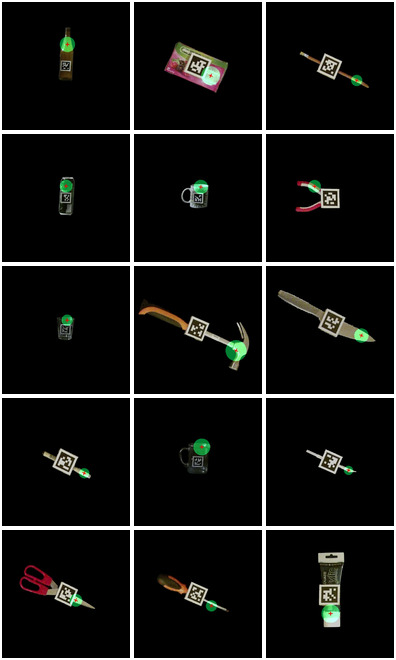
\includegraphics[width=\textwidth]{img/results/objects.jpg}
	\caption{The training objects with the mean values of the corresponding cluster applied to them.}
	\label{fig:results_objects}
\end{figure}

In figure \ref{fig:silhouette_6} we observe two dominant clusters, the first and fourth one. Figure \ref{fig:obj_sample_heatmap} represents a heatmap over the distribution of samples belonging to each object between the clusters. We can see that each cluster represents at least one object, with the exception of the third cluster. The screwdriver, knife, scissors, pen, hammer, scalpell and brush have the largest majority of their samples belonging to the first cluster, while the bottle, pitcher, glass, cup and can are represented by the fourth cluster. The cutters, box and tube are represented by their own clusters, respectively sixth, second and fifth clusters, showing that they are handed over in unique ways compared to the other previous objects. The third cluster seems quite evenly distributed over the objects, with the pitcher having the largest part, which indicates that it can be considered as a cluster of noise from the input data. Table \ref{tab:object_cluster_assign} shows us the final distribution of the objects between the clusters. In figure \ref{fig:results_objects} every object is visualized with their corresponding cluster mean features applied to them.

Already here we can see some similarities between the objects that are clustered together, notable in clusters one and four. The first one includes objects that are longer and thinner and that often include a tip of contact for its usage, like the head of the hammer or the tip of the brush. While the fourth cluster is made of objects that are larger and cylindrical, often used for containing fluids which explains they need to be held similar fashion when handed over as to not spill out the contents.



% ======================================================================================
% CLASSIFICATION
%
% GRAPHS:
%	- loss per step
%	- accuracy per step (validation and testing)
%	- training speed
% TABLES:
%	- confusion matrix
%	- accuracy per object
%	-

\section{Classification}

\subsection{Network configuration}
\label{sec:res_setup}

To summarize the clustering part of this work we are able to divide the objects used for training into a total of five classes. An issue with these results is that three of the classes are represented by a sole item. We judge that it would not be possible to create a balanced dataset to represent equally each class this way. It would also defeat the purpose as to create a model that no longer identifies single object classes, but instead visually similar objects within a same class. Therefore we will discard these three classes and concentrate on the two classes that contain multiple objects. Our network will then be trained for two outputs through a softmax layer.

\begin{table}
	\begin{tabular}{|c|p{5cm}|p{5cm}|}
		\hline
		Class & Training objects & Test objects \\
		\hline
		one & hammer, pen, scalpell, scissors, knife, screwdriver, brush & scissors, fork, knife, spoon, spatula, wooden spoon \\
		\hline
		two & can, pitcher, glass, bottle, cup & bottle, carafe, glass, cup, wine glass, beer glass \\
		\hline
	\end{tabular}
	\caption{Overview of objects included in training set and test set.}
	\label{tab:classification_objects}
\end{table}

In section \ref{sec:testing} we gave a list of objects that are to be used for testing. These were chosen after we made the decision regarding outputs for the network to achieve a balanced dataset over the outputs for testing. Table \ref{tab:classification_objects} shows the distribution of the test objects into classes with the corresponding training objects.


\subsection{Finetuning the network}

\begin{figure}
	\centering
	\begin{subfigure}[b]{\textwidth}
		\input{plot_classification__results-loss}
		\caption{Loss.}
		\label{fig:results_plots_loss}
	\end{subfigure}
	\begin{subfigure}[b]{\textwidth}
		\input{plot_classification__results-val}
		\caption{Validation accuracy.}
		\label{fig:results_plots_val}
	\end{subfigure}
\end{figure}
\begin{figure}
	\ContinuedFloat
	\begin{subfigure}[b]{\textwidth}
		\input{plot_classification__results-test}
		\caption{Test accuracy.}
		\label{fig:results_plots_test}
	\end{subfigure}
	\label{fig:results_plots}
	\caption{Cross entropy, validation and test accuracy during training of the model.}
\end{figure}

\begin{figure}
	\input{plot_classification__confmat}
	\caption{Confusion matrix for k=1.}
	\label{fig:confusion_matrix}
\end{figure}

\begin{table}
	\centering
	\begin{tabular}{l | c | c | c | c}
		\hline
		Set        & Min   & Max   & Mean  & Std.  \\ \hline
		Validation & 0.992 & 1.0   & 0.998 & 0.003 \\
		Test       & 0.886 & 0.922 & 0.906 & 0.013 \\
		\hline
	\end{tabular}
	\caption{Accuracy on the training and test objects for 5 fold cross validation.}
	\label{tab:results_accuracy}
\end{table}

\begin{table}
	\centering
	\begin{tabular}{l | c | c | c | c}
		\hline
		Object       & Min   & Max   & Mean  & Std.  \\ \hline
		Beerglass    & 0.821 & 0.905 & 0.864 & 0.032 \\
		Bottle       & 1.000 & 1.000 & 1.000 & 0.000 \\
		Carafe       & 0.596 & 0.730 & 0.674 & 0.057 \\
		Cup          & 1.000 & 1.000 & 1.000 & 0.000 \\
		Fork         & 1.000 & 1.000 & 1.000 & 0.000 \\
		Glass        & 0.827 & 0.988 & 0.901 & 0.064 \\
		Knife        & 1.000 & 1.000 & 1.000 & 0.000 \\
		Scissors     & 1.000 & 1.000 & 1.000 & 0.000 \\
		Spatula      & 0.940 & 0.964 & 0.955 & 0.009 \\
		Spoon        & 0.976 & 1.000 & 0.993 & 0.010 \\
		Wineglass    & 0.471 & 0.644 & 0.538 & 0.059 \\
		Wooden spoon & 0.926 & 1.000 & 0.951 & 0.027 \\
		\hline
	\end{tabular}
	\caption{Accuracy on individual objects in the test set for 5 fold cross validation.}
	\label{tab:results}
\end{table}

\begin{table}
	\centering
	\begin{tabular}{l | c | c | c}
		\hline
		Class & Precision & Recall & \(F_1\) score \\ \hline
		A     & 0.875     & 0.994  & 0.931 \\
		B     & 0.991     & 0.841  & 0.910 \\ \hline
	\end{tabular}
	\caption{Precision, Recall and \(F_1\) score for the classes.}
	\label{tab:results_precision_recall_f1}
\end{table}


Considering the limited amount of objects that we are using for training the network we run a high risk of overfitting it to these specific objects, and it will not properly classify new ones even though similar. We want the network to recognize the objects in the training set in an abstract fashion as to not learn too much detail about the individual objects. For finetuning the network we therefore chose to train using a larger batch size of 128 and learning rate of 0.0001 for 20 epochs, keeping the initial value of 0.5 for dropout that was used when training the initial weights.

We can see from figure \ref{fig:results_plots_loss} that the network very quickly is able to find zero loss and validation accuracy above 99\%, it however struggles to become steady on the test accuracy. We suspect that is due to some unfortunate overfitting to the training set because we can notice a slight correlation between a lower validation accuracy and higher test accuracy. The graphs for accuracy are also quite irregular between the runs. There is a chance that because of the limitations in data set the network becomes very sensitive to the order that the input is beeing fed for training.

Figure \ref{fig:confusion_matrix} shows us the confusion matrix for the network when it achieved its highest test accuracy of 92.2\% and validation accuracy of 100\%. We obtain a precision of 0.875, recall of 0.994 and an \(F_1\) score of 0.931 for class \(A\) and a precision of 0.992, recall of 0.841 and a \(F_1\) score of 0.91 for class \(B\) (summarized in table \ref{tab:results_precision_recall_f1}). The results tell us that the network is in the end, despite otherwise good results, a little biased towards the first class. This can be explained by the fact that even though the training set is balanced between the classes in terms of number of images per class, it is however not balanced in the number of objects. The first class represents seven objects while the second one only five, meaning that there are more versatile features to learn for the one class than the other.


\begin{figure}
	\centering
	\begin{subfigure}[b]{0.3\textwidth}
		\includegraphics[width=\textwidth]{img/results/bad-images/new-beerglass_100_80.jpg}
		\caption{Beer glass.}
	\end{subfigure}
	\begin{subfigure}[b]{0.3\textwidth}
		\includegraphics[width=\textwidth]{img/results/bad-images/new-carrafe_102_53.jpg}
		\caption{Carafe.}
	\end{subfigure}
	\begin{subfigure}[b]{0.3\textwidth}
		\includegraphics[width=\textwidth]{img/results/bad-images/new-glass_105_43.jpg}
		\caption{Glass}
	\end{subfigure}
	\begin{subfigure}[b]{0.3\textwidth}
		\includegraphics[width=\textwidth]{img/results/bad-images/new-spatula_108_36.jpg}
		\caption{Spatula}
		\label{fig:results_bad_images__spatula}
	\end{subfigure}
	\begin{subfigure}[b]{0.3\textwidth}
		\includegraphics[width=\textwidth]{img/results/bad-images/new-spoon_109_100.jpg}
		\caption{Spoon.}
		\label{fig:results_bad_images__spoon}
	\end{subfigure}
	\begin{subfigure}[b]{0.3\textwidth}
		\includegraphics[width=\textwidth]{img/results/bad-images/new-wineglass_110_22.jpg}
		\caption{Wine glass.}
	\end{subfigure}
	\begin{subfigure}[b]{0.3\textwidth}
		\includegraphics[width=\textwidth]{img/results/bad-images/new-woodenspoon_111_31.jpg}
		\caption{Wooden spoon.}
		\label{fig:results_bad_images__wooden_spoon}
	\end{subfigure}
	\caption{Some images with incorrect predictions.}
	\label{fig:results_bad_images}
\end{figure}


In figure \ref{fig:results_bad_images} we show a sample image of each object that did not achieve 100\% accuracy (a larger sample set can be found in appendix \ref{app:bad_images}). We can observe that the network struggles with objects that are made of glass, especially transparent and thinner glass. This is the case for the carafe, wine glass and beer glass. Other objects in the same class that are not as transparent such as the bottle and the cup, do not have this problem though, and can achieve accuracies of 100\%. This is probably due to the noise and artifacts that appear in the images taken with the depth camera for objects made of thin glass and also the fact they do not have any distinct color they almost become seemingly invisible in some images making them very challenging to identify. Objects in class \(A\) are in one hand quite small in comparison, the network might associate the amount of visible background to this class and when unsure classifying objects that are quite transparent to this class instead. The training set is probably not representative enough of these kind of objects for it to properly learn features to help distinguish them.

A special case is the wine glass, that has the poorest results. Besides the fact that it presents the same challenges as the other glass objects its geometry is also something of a combination of the two classes. Though it has a cylindrical part for liquids it also has a long and thin handle that is similar to for example a pen or brush. As no object in the training set is of the same complex geometry the network as a result has a hard time predicting the correct class for the wineglass.

From the first class there are some objects that did not achieve 100\% accuracy either. From the images of the spatula and the spoon (figures \ref{fig:results_bad_images__spoon} and \ref{fig:results_bad_images__spatula}) there is no object in the other class that we can think that the network confused the objects with, however there is a large amount of noise in these images. We can suspect that the network has learned to associate a degree of noise that is very common in images for glass objects with the second class. On the other hand there are some incorrect predictions that might not always be due to the image quality, as for example the wooden spoon (figure \ref{fig:results_bad_images__wooden_spoon}). One theory to why some of the images of the wooden spoon were incorrectly predicted is that it has some resemblence due to color to the bottle that the network was trained on which is of the opposite class. This shows the limitations of training on such a small dataset of objects that are not versatily represented.


\subsection{Object impact on accuracy}

For the purpose of finding out the impact of each object in the training set on the test accuracy this section will be dedicated to training the network by adding one pair of objects (one object for each class) to the training set and test it's impact on the end results. Table \ref{tab:obj_pairs} summarizes which pairs of objects that were created and the order they were added to the training set. These pairs were chosen randomly. Note that there are only ten objects in total in this test (five for each class), but we have twelwe in total. This is because the dataset is not balanced on objects between classes so we chose to discard two: the \texttt{scalpel} and the \texttt{pen}. These two last objects were chose because they have very similar features that are shared with and represented in the dataset through the \texttt{brush} and in some ways the \texttt{screwdriver}. A more thourough test would be to test all possible permutations of objects to train the network on and evaluate on the test set, but this would be quite time consuming. We therefore rely on this test to give us accurate enough ideas about the impact of each object.

\begin{table}
	\centering
	\begin{tabular}{l | c}
		\hline
		Pair  & Objects \\ \hline
		one   & glass hammer \\
		two   & bottle knife \\
		three & can scissors \\
		four  & pitcher brush \\
		five  & cup screwdriver \\
		\hline
	\end{tabular}
	\caption{Pairs of objects in order they were added to the training set for the network.}
	\label{tab:obj_pairs}
\end{table}

\begin{table}
	\centering
	\begin{tabular}{l | l | c | c | c | c}
		\hline
		\# objects & Set        & Min   & Max   & Mean  & Std.  \\ \hline
		two       & Validation & 0.989 & 1.0   & 0.998 & 0.003 \\
		          & Test       & 0.806 & 0.864 & 0.841 & 0.013 \\ \hline
		four      & Validation & 1.0   & 1.0   & 1.0   & 0.003 \\
		          & Test       & 0.825 & 0.900 & 0.852 & 0.013 \\ \hline
		six       & Validation & 0.992 & 1.0   & 0.997 & 0.003 \\
		          & Test       & 0.835 & 0.925 & 0.880 & 0.013 \\ \hline
		eight     & Validation & 0.995 & 1.0   & 0.998 & 0.003 \\
		          & Test       & 0.940 & 0.956 & 0.944 & 0.013 \\ \hline
		ten       & Validation & 0.996 & 1.0   & 0.998 & 0.003 \\
		          & Test       & 0.936 & 0.978 & 0.961 & 0.013 \\ \hline
	\end{tabular}
	\caption{Accuracy on the training and test objects for 5 fold cross validation.}
	\label{tab:results_perobj}
\end{table}

\begin{figure}
	\input{plot_classification__object-impact}
	\caption{Accuracy for each object depending on how many objects the network is trained on.}
	\label{fig:object_impact}
\end{figure}



\chapter{Conclusions and future work}
\section{Conclusions}

In this work we introduced a model for a system to learn proper handover settings for objects through observations of handovers performed by humans. We showed that we can classify objects depending on a set of features extracted at the moment of the handover. By training a network to output a handover class based on an image of an object we also showed that the objects that have been assigned the same class share similar visual features. Last we showed that these features that have been learned also scale well to other sets of objects that are new to the system.

Based on the features extracted from the handovers, the system is able to cluster the objects and classify them. A handover class will then be defined by a set of features that are to be applied to an object when handing it over. Before clustering we performed PCA to identify the dominant features which were: ratio of object covered by the grasp, direction of vector between center of mass of the object and center grasp in y-axis and in x-axis. Two main classes were identified, where one class contained larger cylindrical objects used for containing for example liquids (cup, glass, bottle, etc.) that were handover in a similar fashion, while objects that are thinner and have a distinct usage area (hammer, pen, scissors) had a different set of features. Outliers in the training set were clustered into their own classes (cutters, box and tube) that contained unique attributes for these objects.

Color and depth images were then taken of the objects from different angles. The blue channel was replaced with the depth image, and then used for training a CNN to recognize the objects and output their respective handover class. The classes that contained only one object were discarded as they would not contain enough data to properly train to identify them. The resulting network was then tested on a different set of images of objects that resembled the training set and manually labeled after the two main classes were created.

Mean performance for our network is 90.6\% with a standard deviation of 1.3\% for objects that were new to the system, while 99.8\% accuracy with a standard deviation of 0.3\% on objects it was trained on. We observed that the network became more biased for the first class than the second, which is likely due to the fact that the two classes were not completely balanced between the objects, suggesting that one class had more versatile features to learn from than the other. We note that the network had a hard time learning to recognize objects made of glass, probably because of troubles with the infrared sensor in the depth camera refracting on the material while taking pictures, making them more challenging to recognize. Objects in the same class but made of other material had results close to 100\%, as well as the objects from the first class which confirms our hypothesis that objects with similar geometry are handed over in similar fashion. In overall the results are quite good considering the small dataset to train on and the artifacts that are created with the depth camera, and with a larger amount of objects and images better results could have probably been achieved. More ideas on how to improve this model are presented in section \ref{sec:future-work}.

\section{Future Work}
\label{sec:future-work}

The results of this work show that a system is able to autonomously learn to handover objects and adapt to novel ones, but some caveats do exist for it to become truly autonomous. The largest problem is object detection, which is a challenging field within computer vision. This work took help of AprilTags to locate and track the objects but in a live environment these tags do not exist on all objects and the system would need a better way of recognizing the object in the handover scene to extract data about the handover. Also in some cases the AprilTag itself could lead to awkward grips of the objects that can lead to incorrect data (see figure \ref{fig:fw_handover_awkward}). Some work show good success using alternatives such as point cloud libraries (\parencite{Chan2015a}). Object detection using point clouds was tried in this work before using AprilTags, but with very poor results. This is something that would need more work to try and implement better without the help of the tags.

\begin{figure}
	\centering
	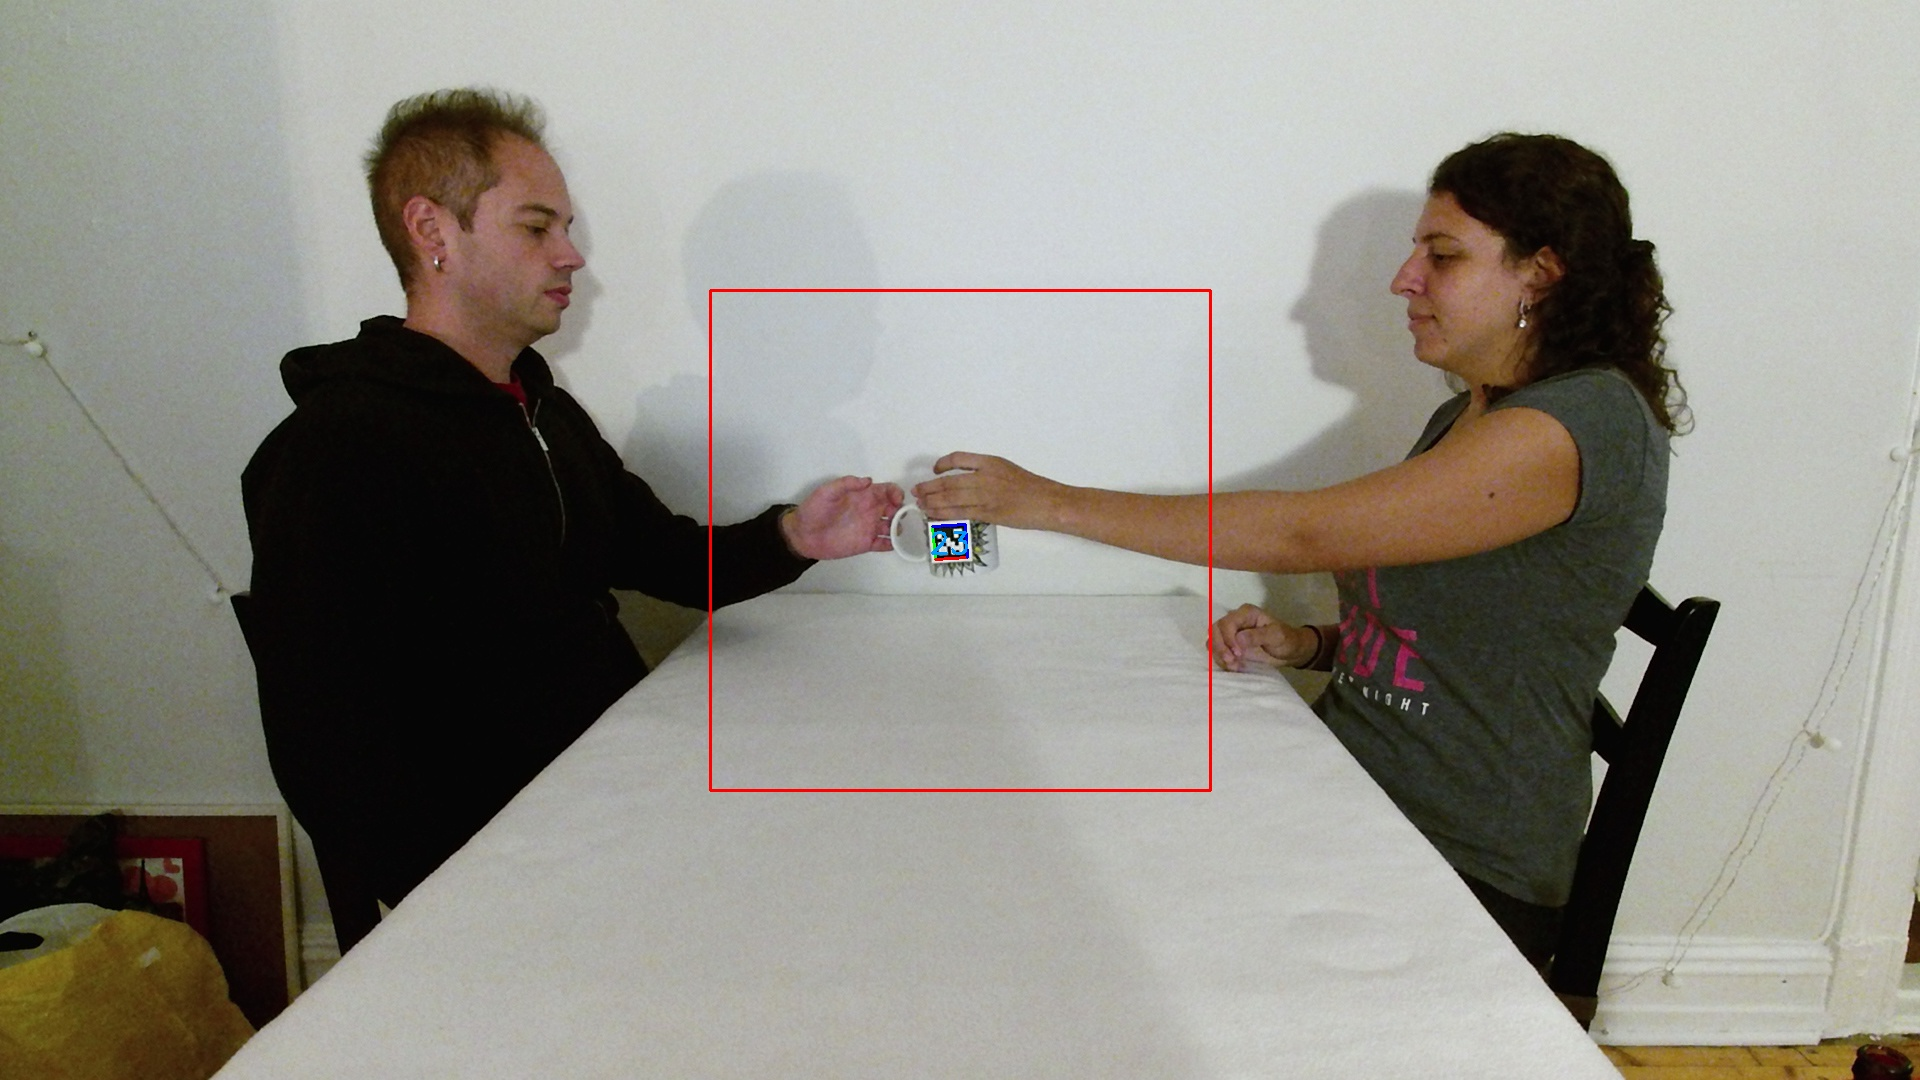
\includegraphics[width=\textwidth]{img/conclusion/awkward_handover_frame.jpg}
	\caption{Some grasps could become unnatural because of the AprilTags.}
	\label{fig:fw_handover_awkward}
\end{figure}

Handover classes from clustering are however not enough to tell a robot how to grasp an object when handing it over. As seen in the results when the settings of one class are applied to an object the grasp region can become outside of it, though rotation and direction from center of object are correct. Future work would have to include calculating more precisely where a robot can grasp the object when handing it over given the data from the handover class.


\printbibliography[heading=bibintoc] % Print the bibliography (and make it appear in the table of contents)

\appendix
\chapter{Unnecessary Appended Material}

\end{document}
